\documentclass[11pt,dvipdfmx,a4paper]{jsarticle}

\usepackage{amsmath,amssymb}
\usepackage{bm}
\usepackage[dvipdfmx]{graphicx}
\usepackage{physics} % http://mirrors.ibiblio.org/CTAN/macros/latex/contrib/physics/physics.pdf
\usepackage{siunitx} %SI単位を楽に出力
\usepackage{mathtools} %環境の追加
% \usepackage{circuitikz} %電気回路をtex中で書く
% \usepackage{caption} %番号なしキャプションを書く
% \usepackage{cancel} %式中に斜線を入れる
% \usepackage{tensor} %テンソルの添え字を書く
\usepackage{tikz} %図を書く
% \usepackage{ascmac} %四角い枠の中に文章を書く
% \usepackage{float} %figureで[hbp]オプションを使う
% \usepackage{hyperref}  \usepackage{pxjahyper} %ハイパーリンクをつかう
% \usepackage{tablefootnote} %表中に注釈をいれる
% \usepackage[thicklines]{cancel} %数式中の取り消し線
\usepackage[version=4]{mhchem} %化学式の入力
\usepackage{pdfpages}
% \usepackage{wrapfig} %文章の回り込み
\usepackage[subrefformat=parens]{subcaption} %(a)図のようにすることができるやつ
\usepackage{here}
\usepackage{url}
\usepackage[margin=15mm]{geometry} %余白の削除

\newcommand{\cc}{\text{(C.C.)}}

\graphicspath{{./image/}}

\begin{document}

%出力したpdfを表紙にするとき
% \includepdf[pages=1,noautoscale=false]{cover.pdf}
% \newpage

%texで表紙を書くとき
\quad\\[35mm]
\centerline{\Huge{\textsf{第 3 回}}}
\quad\\[5mm]
\centerline{\Huge{\textsf{応 用 物 理 学 実 験}}}
\quad\\[5mm]
\begin{table}[h]
	\centering
	\begin{tabular}{| c | c |}
		\hline
		\Huge\textsf{{題目}} & \Huge{\textsf{核磁気共鳴}} \rule[-5mm]{0mm}{15mm} \\
		\hline
	\end{tabular}
\end{table}
\quad\\[10mm]
\begin{table}[h]
	\centering
	\begin{tabular}{l l}
		\hline
		\LARGE{\textsf{氏\qquad 名}} & \LARGE{\textsf{: 西原 翔}} \rule[0mm]{0mm}{6mm} \\
		\hline
		\LARGE{\textsf{学  籍  番  号}} & \LARGE{\textsf{: 1522068}} \rule[0mm]{0mm}{6mm} \\
		\LARGE{\textsf{学部学科学年}} & \LARGE{\textsf{: 理学部第一部応用物理学科3年}}\\
		\hline
	\end{tabular}
\end{table}
\quad\\[10mm]
\centerline{\LARGE{\textsf{共同実験者:1522064 中井空弥}}}\\[2mm]
\centerline{\LARGE{\textsf{\qquad\qquad\quad\;\;1522091 宮田祟杜}}}\\[2mm]
\centerline{\LARGE{\textsf{\qquad\qquad\quad\;\;1522095 村山涼矢}}}\\[2mm]
\centerline{\LARGE{\textsf{\qquad\qquad\quad\;\;1522B02 中村洸太}}}\\[2mm]
\quad\\[10mm]
\centerline{\LARGE{\textsf{提出年月日:2024年06月13日}}}\\[2mm]
\centerline{\LARGE{\textsf{実験実施日:2024年05月31日}}}\\[2mm]
\centerline{\LARGE{\textsf{\qquad\qquad\quad\;2024年06月07日}}}
\quad\\[10mm]
\centerline{\LARGE{\textsf{東 京 理 科 大 学 理 学 部 第 1 部}}}\\[2mm]
\centerline{\LARGE{\textsf{応 用 物 理 学 教 室}}}

\thispagestyle{empty}
\clearpage
\addtocounter{page}{-1}
\newpage

% \twocolumn
\section{目的}
量子は外部磁場のもとでは量子は Zeeman 効果によりエネルギー準位が分裂する。
さらにその分裂した準位のうち2つの準位と共鳴するような電磁波を入射すると、
誘導吸収・誘導放出により分裂した準位間で光子を吸収したり放出したりして量子が周期的に遷移するようになる。
これを Rabi 振動という。
とくに原子核のエネルギー準位の Zeeman 分裂に外部振動磁場を入射して共鳴させるのを
核磁気共鳴(Nuclear magnetism Resonance, NMR) と呼ぶ。

静磁場により2エネルギー準位が2つに分裂した状態で、
振動外場をパルス的に入射すると、
量子状態は基底準位と励起準位の重ね合わせ状態にすることができる。
これは古典電磁気学的な描像だと、原子核スピンは乱雑な向きを持つ状態とみなせる。
この状態はいつまでも続くわけではなく、原子核の置かれた環境系と相互作用していき、
熱平衡状態へと緩和する。
その際、原子核スピンの周囲に緩和時間の速い電子スピンがある、言い換えると原子が磁性を持っているとき、
はじめにかけた静磁場に加え電子スピンによる磁場が加わるため、原子核スピンの緩和時間も短くなる。
また、周囲に電子スピンがなかったとしてもかけた静磁場の不均一さや周囲の原子核スピンによる磁場による緩和時間の変化もある。
この緩和の様子を調べることで原子核の周りにある系の性質を調べることができる。

この実験では純水、塩化ナトリウム水溶液、硫酸銅水溶液、硫酸亜鉛水溶液、硫酸鉄(II)水溶液の緩和の様子や磁性を
水素原子核の核磁気共鳴状態からの緩和の様子を通して調べた。
また緩和のある Bloch 方程式の解の振る舞いを量子情報の観点から分析をした。

\section{原理}
\subsection{\(g\) 因子}
古典電磁気学によると質量\(m\)で角運動量\(\vb*{J}\)を持ち電荷\(q\)を持つ粒子は磁気モーメント\(\vb*{\mu}\)を持ち、
\begin{equation}
	\vb*{\mu} = \frac{q}{2m} \vb*{J}
\end{equation}
となる。

量子が持つ内部自由度にはスピンというものがありこれは角運動量を持つため、
スピンは磁気モーメントとなる。
しかしスピンの持つ磁気モーメントは古典電磁気学の結果とは違う。
角運動量を\(\hbar\vb*{S}\)とすると比例定数\(g\)を用いて
\begin{equation}
	\vb*{\mu}_z = g\frac{q\hbar}{2m} \vb*{S}_z
\end{equation}
となる。この比例定数を\(g\)因子という。
電子の\(g\)因子は\(g \simeq -2.0\)で、電子は電荷\(-e\), スピン角運動量は\(\hbar/2\)であるので磁気モーメントは
\begin{equation}
	\mu_B = \frac{e\hbar}{2m_e}
\end{equation}
となる。これをボーア磁子という。
今回の実験では水素原子核、つまり陽子の磁気モーメントを調べる。
原子核スピンの\(g\)因子は同様に
\begin{equation}
	\mu = g \frac{q}{2m} S
\end{equation}
で定義される。

\subsection{Zeeman 分裂}
量子系を半古典論で扱う時、外部磁場は摂動として
\begin{equation}
	\hat{\mathcal{H}}_1 = -\hat{\vb*{\mu}}\cdot \vb*{H}
\end{equation}
というように表わされる。
磁気モーメント演算子は磁気回転比\(\gamma = gq/2m\)を用いると、
\begin{equation}
	\hat{\vb*{\mu}} = \frac{ge}{2m}\hat{\vb*{J}} = \gamma\frac{\hat{\vb*{J}}}{\hbar}
\end{equation}
というように表わされる。
今回行う H-NMR の系では水素原子核である陽子のスピンの状態を扱う。
陽子の角運動量は\(J=\pm\hbar/2\)である。
磁場は\(z\)成分しかないものと考えてやると、
始めに静磁場\(H_0\)をかけたときの 1 次の摂動エネルギーは
\begin{equation}
	E_1 = \pm\frac{\gamma\hbar H_0}{2}
\end{equation}
というようになる。
% (付録:摂動論) % TODO 一次の摂動論のエネルギー
よって Zeeman 効果によるエネルギー準位の分裂幅\(\hbar\omega_0\)は
\begin{align}
	\hbar\omega &= \hbar \gamma H_0\\
	\omega_0 &= \gamma H_0
\end{align}
というようになる。
分裂したエネルギー準位のうち、エネルギーが低い方の準位は静磁場と同じ向きを向いた方向である。

\(\omega_0\)は分裂したエネルギー準位の共鳴周波数となっている。
これより振動数\(\omega_0\)の外場を加えると共鳴状態となり Rabi 振動を起こす。
% 外部磁場の強さに対する磁気モーメントの歳差運動の周波数を関係づける式とみなせる。 % (付録)

\subsection{Rabi 振動}
H-NMR におけるスピンの量子力学的状態は Bloch ベクトル\(M = (x,\,y,\,z)\)で表され、
共鳴状態における Bloch ベクトルの時間発展は Bloch 方程式
\begin{equation}
	\dv{t}
	\begin{pmatrix}
		x\\ y\\ z
	\end{pmatrix}
	=
	\begin{pmatrix}
		-\gamma & -(\omega-\omega_0) & 0\\
		\omega -\omega_0 & -\gamma & -2\gamma_p H\\
		0 & 2\gamma_p H & -\Gamma
	\end{pmatrix}
	\begin{pmatrix}
		x\\ y\\ z
	\end{pmatrix}
\end{equation}
で記述される(付録 : Bloch 方程式の導出)。
ここで
\(\omega\)は入射した振動磁場の周波数、\(\omega_0\)は共鳴周波数、
\(\gamma_p\)は陽子の磁気回転比、\(H\)は振動外部磁場の強さである。
また\(\gamma\)は横緩和、\(\Gamma\)は縦緩和という量で、
前者は弾性散乱によりスピンの状態が乱されるデコヒーレンスの速さを表す量で、
後者は非弾性散乱により、励起した準位の持つエネルギーが熱になってを失っていく速さをを表している。 % TODO たぶん嘘言ってる。
Bloch ベクトルは古典的な描像としてスピンの持つ磁気モーメントの向く方向とみなすこともできるのでこれら2つの描像を使っていく。

\begin{figure}[htb]
	\centering
	\begin{minipage}[t]{0.48\columnwidth}
		\centering
		\tikz{
			\tikzstyle{st}=[gray, fill, fill opacity=0.1]
			\coordinate(o)at(0,0);
			\draw(o)circle(2cm);
			\draw[fill](o)circle(1.5pt);%origin
			\draw[st](o)--(90:0.6)arc(90:150:0.6)--cycle;%theta angle
			\draw(-0.6,0.9)node[fill=white]{$\tiny{2\gamma_p Ht}$};
			\draw[->](o)--(224.28:1.5) node[below left]{$x$};%x
			\draw[->](o)--(2.5,0)node[right]{$y$};%y
			\draw[->](o)--(0,2.5)node[below right]{$z$};%z
			\draw[rotate around={0.:(0.,0.)},dashed](0,0)ellipse(2cm and 0.9cm);%ellipse
			\draw[thick,->](o)--(150:2)node[above left]{$\vb*{M}$};%state vector
			\draw[thick,->](o)--(224.28:1.1)node[above=3mm]{$\vb*{\tilde{H}}$};%rotate axis vector
			\draw[densely dotted,-](o)--(0,-2);
			}
			\subcaption{初期状態\(\vb*{M}=(0,\,0,\,1)\)から大きさが\(H\)の共鳴外部磁場を入射して\(t\)秒後の水素原子核のスピンの状態を Bloch 球で表したもの。
			共鳴磁場をかけたときには\(\vb*{\tilde{H}}=(H,\,0,\,0)\)なので状態\(\vb*{M}\)は\(x\)軸を回転軸として
		振動数\(2\gamma_p H\)で回転(振動)する。}
		\label{fig:Rabi_X}
		\end{minipage}
	\hfill
	\begin{minipage}[t]{0.48\columnwidth}
		\centering
		\tikz{
			\tikzstyle{st}=[lightgray, fill, fill opacity=0.1]
			\coordinate(o)at(0,0);
			\draw(o)circle(2cm);
			\draw[fill](o)circle(1.5pt);%origin
			\draw[st](o)--(-135.7:0.6)arc(-135.7:-159:0.6)--cycle;%varphi angle
			\draw(-0.9,0.1)node{$-\omega_0t$};
			\draw[->](o)--(224.28:1.5) node[below left]{$x$};%x
			\draw[->](o)--(2.5,0)node[right]{$y$};%y
			\draw[->](o)--(0,2.5)node[below right]{$z$};%z
			\draw[rotate around={0.:(0.,0.)},dashed](0,0)ellipse(2cm and 0.9cm);%ellipse
			\draw[thick,->](o)--(-1.2,1.07)node[above]{$\vb*{M}$};%state vector
			\draw[thick,->](o)--(0,-1.8)node[above right]{\(\vb*{\tilde{H}}\)};
			\draw[densely dotted,-](o)--(0,-2);
			\draw[dotted](o)--(-1.2,-0.46)--(-1.2,1);%triangle
		  }
		\subcaption{始状態が\(\vb*{M} = (\sin\theta_0,\,0,\,\cos\theta_0)\)の水素原子核のスピンが
		外部振動磁場のない条件で\(t\)秒経った時の状態を Bloch 球で表したもの。
		このとき\(\vb*{\tilde{H}} = (0,\, 0,\, -\omega_0)\)なので状態\(\vb*{M}\)は\(z\)軸を回転軸として
		振動数\(-\omega_0\)で回転する。}
		\label{fig:Rabi_Z}
	\end{minipage}
	\caption{緩和がないときの Bloch 方程式の解の示すスピンの状態の変化を Bloch 球上で表したもの。}
	% https://qiita.com/ThomsonKernel/items/1b105370fb5ce94b2cd3
\end{figure}

まずは熱揺らぎがなく、スピンが基底状態に確実にあって、緩和のないときを考える。
すると Bloch 方程式は振動数\(\omega_0\)
で回転する系における見かけの磁場
\begin{equation}
	\gamma_p \vb*{\tilde{H}} = \qty(2\gamma H,\,0,\,\omega-\omega_0)
\end{equation}
を用いて
\begin{equation}
	\dv{\vb*{M}}{t} = \gamma_p \vb*{\tilde{H}} \times \vb*{M}
\end{equation}
と書ける。

この方程式の振舞いについて考える。
はじめ静磁場がかかっているときにはスピンの向きはすべて上向きで揃っているので
始状態は\(\vb*{M}=(0,\,0,\,1)\)
である。
このとき、振動磁場ははかかっていないので\(\vb*{\tilde{H}}=(0,\,0,\,-\omega_0)\)
となり、磁場とスピンの向きが揃っているため状態は状態の時間微分は0で状態は変化せず一定のままとわかる。

つぎに共鳴磁場を入れたときには\(\vb*{\tilde{H}}=(H,\,0,\,0)\)となり、
磁場とスピンの向きが直交するため時間変化を始める。その解は
\begin{equation}
	(x,\,y,\,z) = \qty(0,\,-\sin(2\gamma_p Ht),\,\cos(2\gamma_p Ht))
\end{equation}
というように\(x\)軸を軸として回転していく(図\ref{fig:Rabi_X})。
これを量子力学的なエネルギー準位の描像で見ると、
共鳴磁場を入れたとき Zeeman 分裂した2準位の基底状態と励起状態を行き来しているのがわかる。
これを Rabi 振動といい、振動数\(2\gamma_p H\)を Rabi 周波数と呼ぶ。

共鳴磁場を切った後の状態の変化を考える。
始状態が\(\vb*{M}=(\sin\theta_0,\,0,\,\cos\theta_0)\)のとき、Bloch 方程式を解くと
\begin{equation}
	(x,\,y,\,z) =
	\qty(\sin\theta_0\cos(-\omega_0 t),\,
	\sin\theta_0\sin(-\omega_0 t),\,\cos\theta_0)
\end{equation}
というように\(z\)軸を中心として回転するようになる(図\ref{fig:Rabi_Z})。
量子力学的な描像では基底状態と励起状態の重ねあわせ状態になっている。
もう少し詳細な描像である密度演算子を用いて考えると、これは非対角成分が最大の状態である。
つまりもっとも多く基底準位と励起準位の間を誘導吸収・誘導放出をしている状態である(付録:線形感受率)。
これは実際の現象にはどうゆう風に現れるかというと、
磁気双極子の大きさの時間変化が大きく放出する光子が多くなるため、
観測する応答磁場の振幅が強くなることを表す。この状態を飽和状態と以降呼ぶ。

緩和 のない Bloch 方程式の振る舞いを見たことで NMR の実験系を考える上で大事なことが分かった。
それは共鳴磁場を入れる時間によってスピンの\(z\)成分の大きさや、
共鳴により系が放出する磁場の強さを指定することができることである。

スピンの向きが下向きの励起状態にしたいときには、
スピンの向きが上向きの揃っている基底状態となっている時刻から、
共鳴磁場を入れて\(x\)軸を回転軸として\(t=2\gamma_pH/\pi\)の時間回転させる。
その後共鳴磁場を切ると\(z\)軸を回転軸として回るようになるが、
スピンの向きは\(z\)軸を向いているため状態はずっと励起状態になる。
スピンを基底状態と励起状態の重ね合わせ状態にさせたい、
もしくは飽和状態にして共鳴信号をはっきりと見たいときには、
スピンの向きが上向きに揃っている基底状態となっている時刻から
共鳴磁場を入れて\(x\)軸を回転軸として\(t=\gamma_pH/\pi\)の時間回転させる。
その後共鳴磁場を切ると\(x-y\)平面の円周上のを回るようになる。
前者の操作を\(\pi\)パルス、後者の操作を\(\pi/2\)パルスという。
また回転させる天頂角\(\theta\)をパルス面積と言ったりする。

今回の実験では\(\pi/2\)パルスを入れた状態の縦緩和を見ていくことになる。

\subsection{状態の緩和}
緩和を考えない Bloch 方程式では一度共鳴磁場を入れてそれを切るとスピンの\(z\)成分は保存されるのであったが、
実際にはスピンの外部の系との相互作用により熱平衡状態へ緩和していくことが予想される。

熱平衡状態における状態\(\vb*{M}=(0,\,0,\,z_{1})\)について考える。
熱平衡状態ではボルツマン分布を考えると
基底準位にいる確率\(\rho_{gg}\)と励起準位にいる確率\(\rho_{ee}\)は
\begin{equation}
	\rho_{gg} = \frac{1}{1 + e^{-\beta \hbar\omega_0}} \qquad
	\rho_{ee} = \frac{1}{1 + e^{\beta \hbar\omega_0}}
\end{equation}
となっている。
\begin{equation}
	z = \rho_{gg} - \rho_{ee}
\end{equation}
なので熱平衡状態における状態は
\begin{equation}
	z_{1} = \tanh{\frac{\beta\hbar\omega_0}{2}}
\end{equation}
というようになる。低温極限では\(z_{1}=1\), 高温極限では\(z_{1} = 0\)である。

緩和のある Bloch 方程式を解くと、始状態\(\vb*{M}=\qty(x_0,\,y_0,\,z_0)\), 熱平衡状態を\((0,\,0,\,z_{1})\)
として
\begin{equation}
	\left\{\quad
	\begin{aligned}
		x(t) + iy(t) &= (x_0 + iy_0) e^{i(\omega-\omega_0)t}e^{-\gamma t}\\
		z(t) &= z_0 e^{-\Gamma t} + z_{1}(1-e^{-\Gamma t})
	\end{aligned}\right. \label{eq:relaxed_Bloch_sol}
\end{equation}
が得られる。
この式の形を見ると\((x,\,y)\)はまとめて複素数\(\xi = x + iy\)とおいてやると見やすくなるので、
以降\(\vb*{M}=(\xi,\,z)\)と書いたりする。
これより縦緩和\(\Gamma\)と横緩和\(\gamma\)の意味が分かりやすくなる。

\(\Gamma\)が大きいと状態ベクトルの\(z\)成分が \(z_1\) の熱平衡状態へと緩和する時間が短くなる。
これは縦緩和は振動外場によって原子核が得たエネルギーが失われていってこれ以上落ち込むことのできない
熱ゆらぎも考慮した基底準位になる過程を表す。
この緩和の要因としては原子核の周りにある電子のスピンによる磁性などがある。% TODO 確認する

横緩和については少しわかりくい。
これは原子核1つのスピンを考えるのではなく、系全体のスピンの向く方向を考えるとよい。
始め\(\vb*{M}=(0,\,1)\)にあったスピンはすべて\(\pi/2\)パルスにより
\(\vb*{M}=(1,\,0)\)の方向へと向く。
それぞれのスピンはエネルギー変化を伴わない弾性散乱をランダムに受け、
そのため\(z\)軸の回転する速さというのは各スピンでばらけてくる。
実際に測定するのは1つのスピンではなく系全体のスピンの平均となるため、
ばらけた方向を向くスピンの大きさが 0 へと向かっていくことになる。
系全体のスピンの向きのそろい具合をコヒーレンスといい、
横緩和はこのコヒーレンスが失われる速度を表していることがわかる。

\subsection{緩和の測定}
緩和した状態の様子の測定法を考える。
\(\gamma\gg\Gamma\)であることが知られている。
これより\(\pi/2\)パルスを打ち飽和状態の縦緩和を見ようとすると、
縦緩和の時間スケールでは横緩和が速すぎるためすぐさま\(\vb*{M}=(0,\,0,\,0)\)の状態になる。
その状態から縦緩和が生じていき、縦緩和の時定数を\(T_1 = 1/\Gamma\)
熱平衡状態における状態の\(z\)成分を\(z_1\)とすると状態は
\begin{equation}
	\vb*{M}(t) = \qty(0,\,0,\,z_1(1-e^{-t/T_1}))
\end{equation}
となる。
始めに\(\pi/2\)パルスを入れてから\(t_j\)秒後の状態を考える。
そのときもう一度\(\pi/2\)パルスをかけ、
今度は横緩和の時定数\(T_2=1/\gamma\) のスケールで考えると系の状態は
\begin{equation}
	\vb*{M}(t+t_j) = \qty(z_1(1-e^{-t_j/T_1}\cos(\omega-\omega_0 t)e^{-t/T_2}),\,
	z_1(1-e^{-t_j/T_1}\sin(\omega-\omega_0 t)e^{-t/T_2}),\,0)
\end{equation}
というようになる。
スピンの持つ磁気モーメント\(\mu\)は状態\(\vb*{M}\)の\(x\)成分に比例する。
つまり
\begin{equation}
	\mu(t) \propto z_1(1-e^{-t_j/T}\cos(\omega-\omega_0 t)e^{-t/T_2}). \label{eq:MD_T2_ev}
\end{equation}
磁気モーメントが時間変化すると双極子放射により電磁波を放出するようになる。
双極子放射はスピンの方向である\(z\)軸と垂直な方向に電磁波を発するため、
この方向に電磁波を測定するような仕組みを用意してやれば系の状態を測定することができる。
今回の実験では始めにかける静磁場と垂直な方向にソレノイドコイルをセットし、
その内部に試料を入れることで、NMR から出た磁場をソレノイドが感じる変動磁場として電気信号に変えて測定する。


\subsection{ホモダイン検出・ロックイン検出}
(\ref{eq:MD_T2_ev}) 式が NMR 信号として現れるとあったが、
これは\(\omega_0\)で回転している系での周波数である。
そのため実際に測定されるのは入射したパルスの振動数\(\omega\)
とほとんど同じ周波数として出力される。
\(\omega-\omega_0\)の値は\(\omega_0\)に比べてとても小さいため、
測定法に工夫が必要となる。それがホモダイン検出・ロックイン検出である。
大雑把に説明すると、これは入力パルスをNMRだけではなく信号の測定装置にも伝え、
出力と入力の信号の積をとるような信号測定の手法である(参考文献\cite{Morita_2010})。


\section{実験}
実験室に備えられている NMR 装置を用いて試料に含まれている水素原子核スピンの緩和を用いて、
試料のもつ物性について測定した。
\subsection{測定試料}
水溶液に溶けている溶質の量と核磁気共鳴の緩和時間の関係を見るため
硫酸銅(II)水溶液の濃度を
\(5\times 10^{-3}\) mol/L,
\(10\times 10^{-3}\) mol/L,
\(20\times 10^{-3}\) mol/L
の三通りで測定を行った。
またこの結果を利用して水素原子核スピンの磁気モーメントの大きさを測定した。

核磁気共鳴の緩和時間によって水素原子核の周囲の環境がわかることを利用して、
\(5\times 10^{-3}\) mol/L の硫酸銅(II)水溶液に
塩化ナトリウム、硫酸亜鉛、硫酸鉄(II)
をそれぞれ加え、これら試料を入れなかったときの緩和時間と比較した。
磁性が何もないと予想される純水の核磁気共鳴の緩和の出力信号を記録し縦緩和と横緩和について調べた。

\subsection{装置の概要}
実際の測定装置は図\ref{pic:machine}である。
試料は溶液であるため試験管に入れて、
装置に取り付けたソレノイドコイルにセットしておく。
\begin{figure}[H]
	\centering
	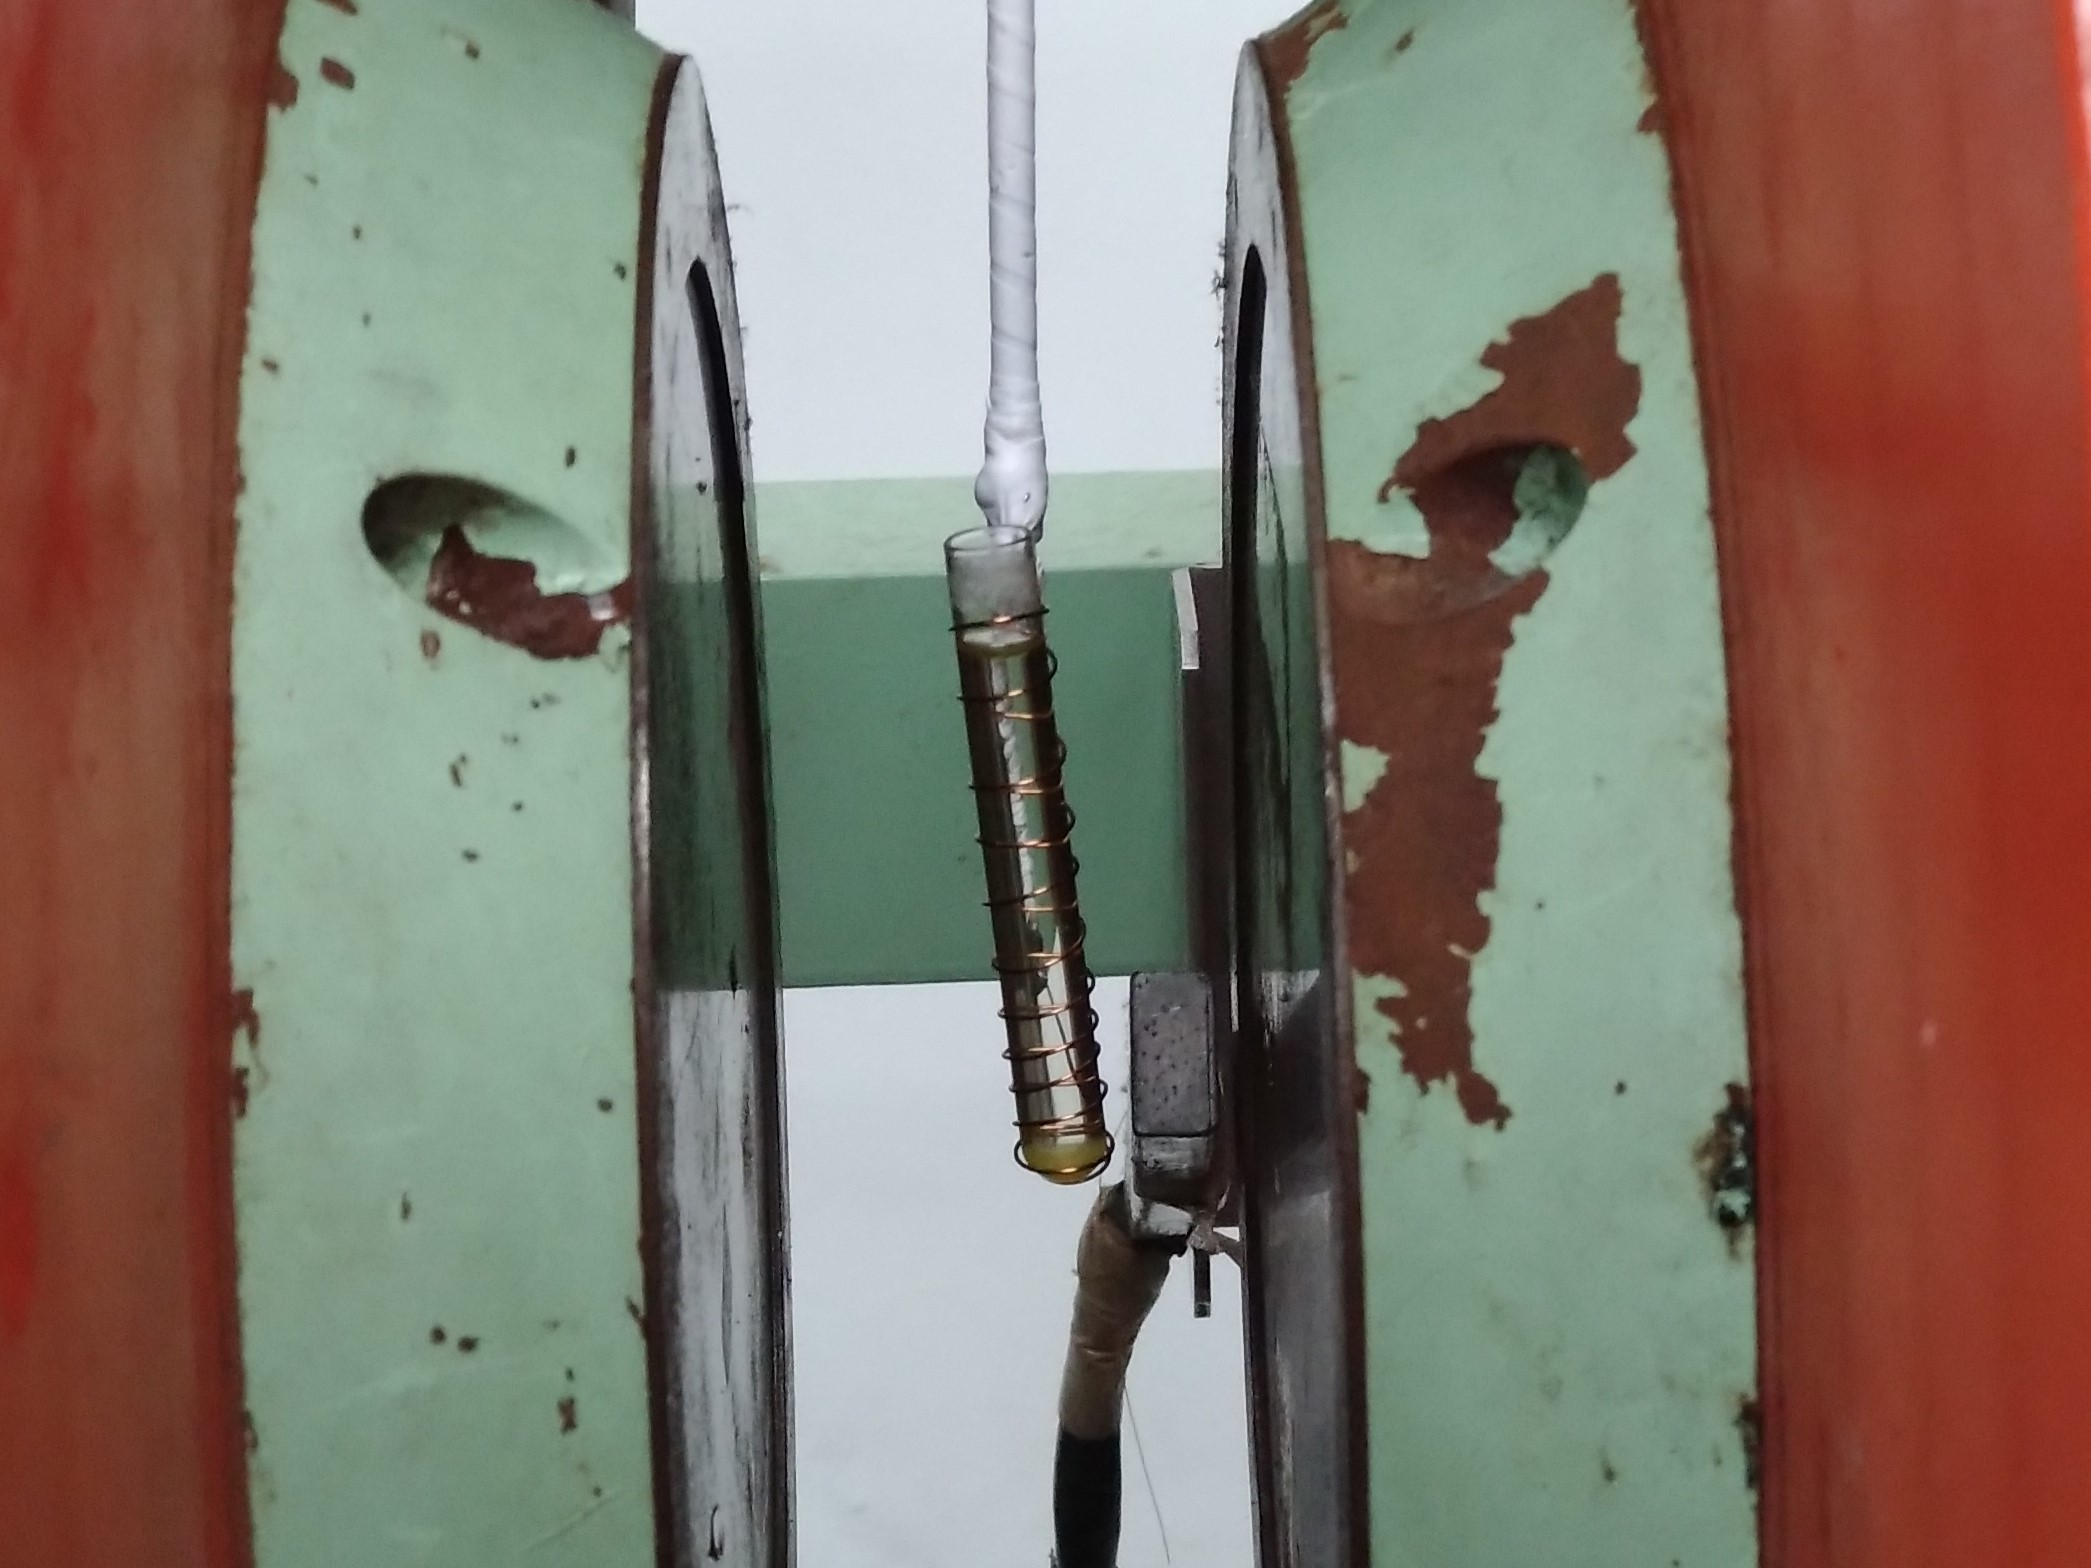
\includegraphics[width=0.5\columnwidth]{/pic/01.JPG}
	\caption{実際の使用した装置。
	左右にある電磁石によって静磁場をかけ、Zeeman 分裂をさせる。
	静磁場と垂直な方向にソレノイドコイルをセットし、入力信号と出力信号をここから入れる。
	ソレノイドコイルの中には試験管とこれに入れられた試料が入っている。}
	\label{pic:machine}
\end{figure}

静磁場は電磁石によって発生させ、これによって水素原子核のエネルギー準位を Zeeman 分裂をさせた。
電磁石であるため、流す電流によって磁場の強さを変えることができる。
流した電流と静磁場の大きさはの関係式は電磁石の中心部では
\begin{equation}
	H (\text{T}) = 0.01058 (\text{T/A}) \times I (\text{A})
\end{equation}
で与えられる。

ソレノイドコイル内部にかかる磁場はコイルを流れる電流に比例するので、
入力パルス信号を交流電流としてソレノイドコイルに入れ、
ソレノイドコイル内部の磁場として試料に振動磁場を加えた。
NMR の縦緩和を調べるのが目的であるため、
初めに\(\pi/2\)パルスをいれ、\(t_j\)秒縦緩和させたあとまた\(\pi/2\)パルスを入れた。
そうして得られた NMR 信号をホモダイン測定するとある波形が得られる。
この波形は横軸が横緩和の時間スケールで、
縦軸が磁気モーメントの大きさを表し、磁気モーメントの振幅の大きさとして縦緩和が見ることができる。

\section{結果}

硫酸銅(II)水溶液の濃度を変えた時の縦緩和の様子は図\ref{graph:T1_con}のようになった。
濃度が上がれば上がるほど緩和が速くなっているのがわかる。
硫酸銅(II)水溶液に塩化ナトリウム、硫酸亜鉛、硫酸鉄(II) を入れたときの縦緩和の様子は図\ref{graph:T1_var}のようになった。
塩化ナトリウムを加えたものは緩和が少し遅くなり、硫酸鉄(II) を加えたものは緩和がとても速くなったのがわかる。

純水の横緩和の様子は図\ref{graph:water_ex}のようになった。
この測定データにはノイズが多いため、
減衰振動となっている部分のデータを用いてフィッティングを行ったのが図\ref{graph:water_fit}である。
またこのフィッティングにより減衰振動の振幅として現れる縦緩和をプロットしたのが図\ref{graph:T1_water}である。
縦緩和の時間スケールが硫酸銅水溶液を用いた時に比べ桁違いに遅いことがわかる。
その他このデータ振舞いは考察にて触れる。
こうして得られたデータを解析して得られた試料の縦緩和の緩和時間は表\ref{table:relax}のようになった。
\begin{figure}[h]
	\centering
	\begin{minipage}[t]{0.48\columnwidth}
		\centering
		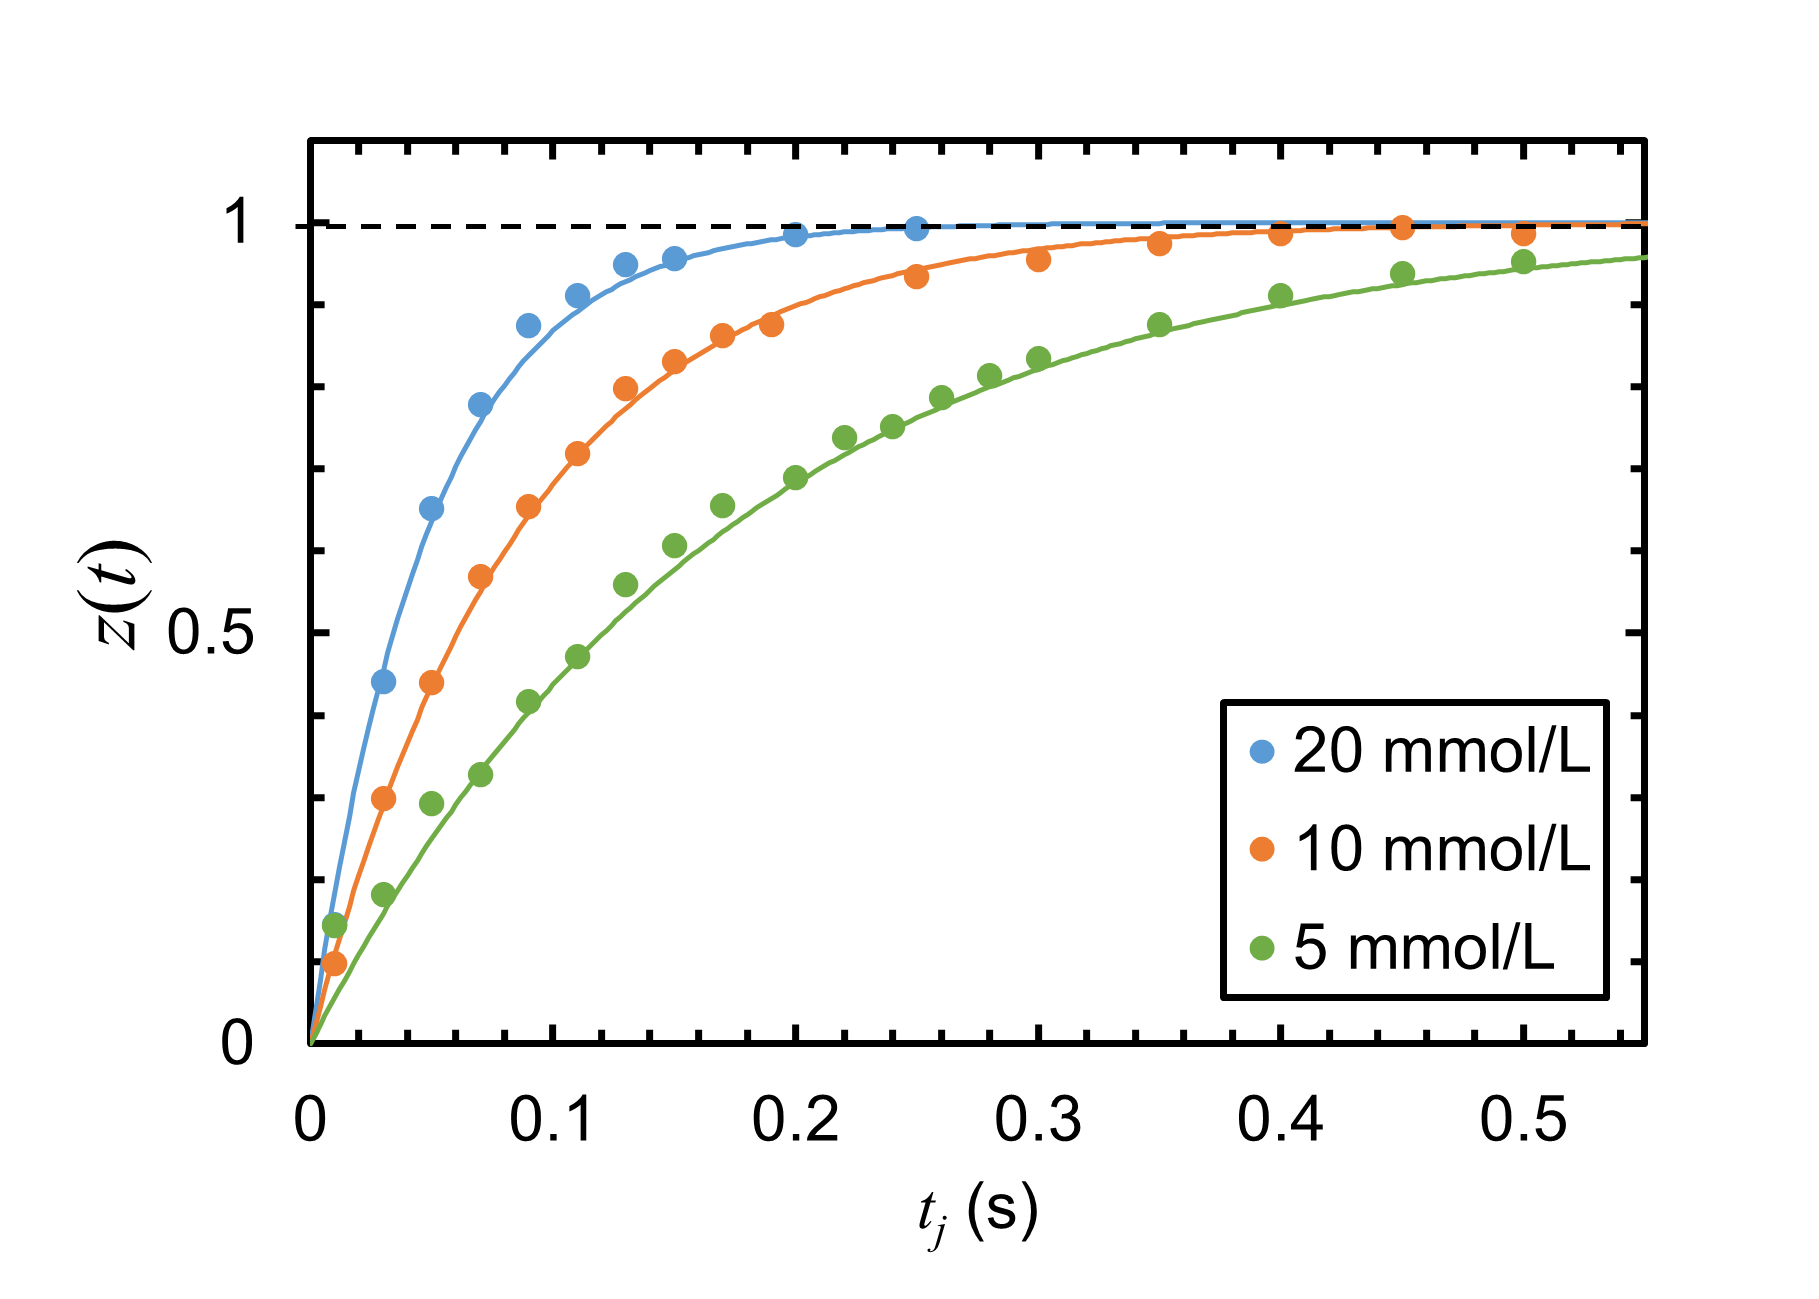
\includegraphics[width=\columnwidth]{graph/T1_con.png}
		\caption{\ce{CuSO4}水溶液の濃度を変えたときの縦緩和の様子。
		縦軸が状態\(\vb*{M}\)の\(z\)成分を表し、横軸が縦緩和の時間を表している。}
		\label{graph:T1_con}
	\end{minipage}
	\hfill
	\begin{minipage}[t]{0.48\columnwidth}
		\centering
		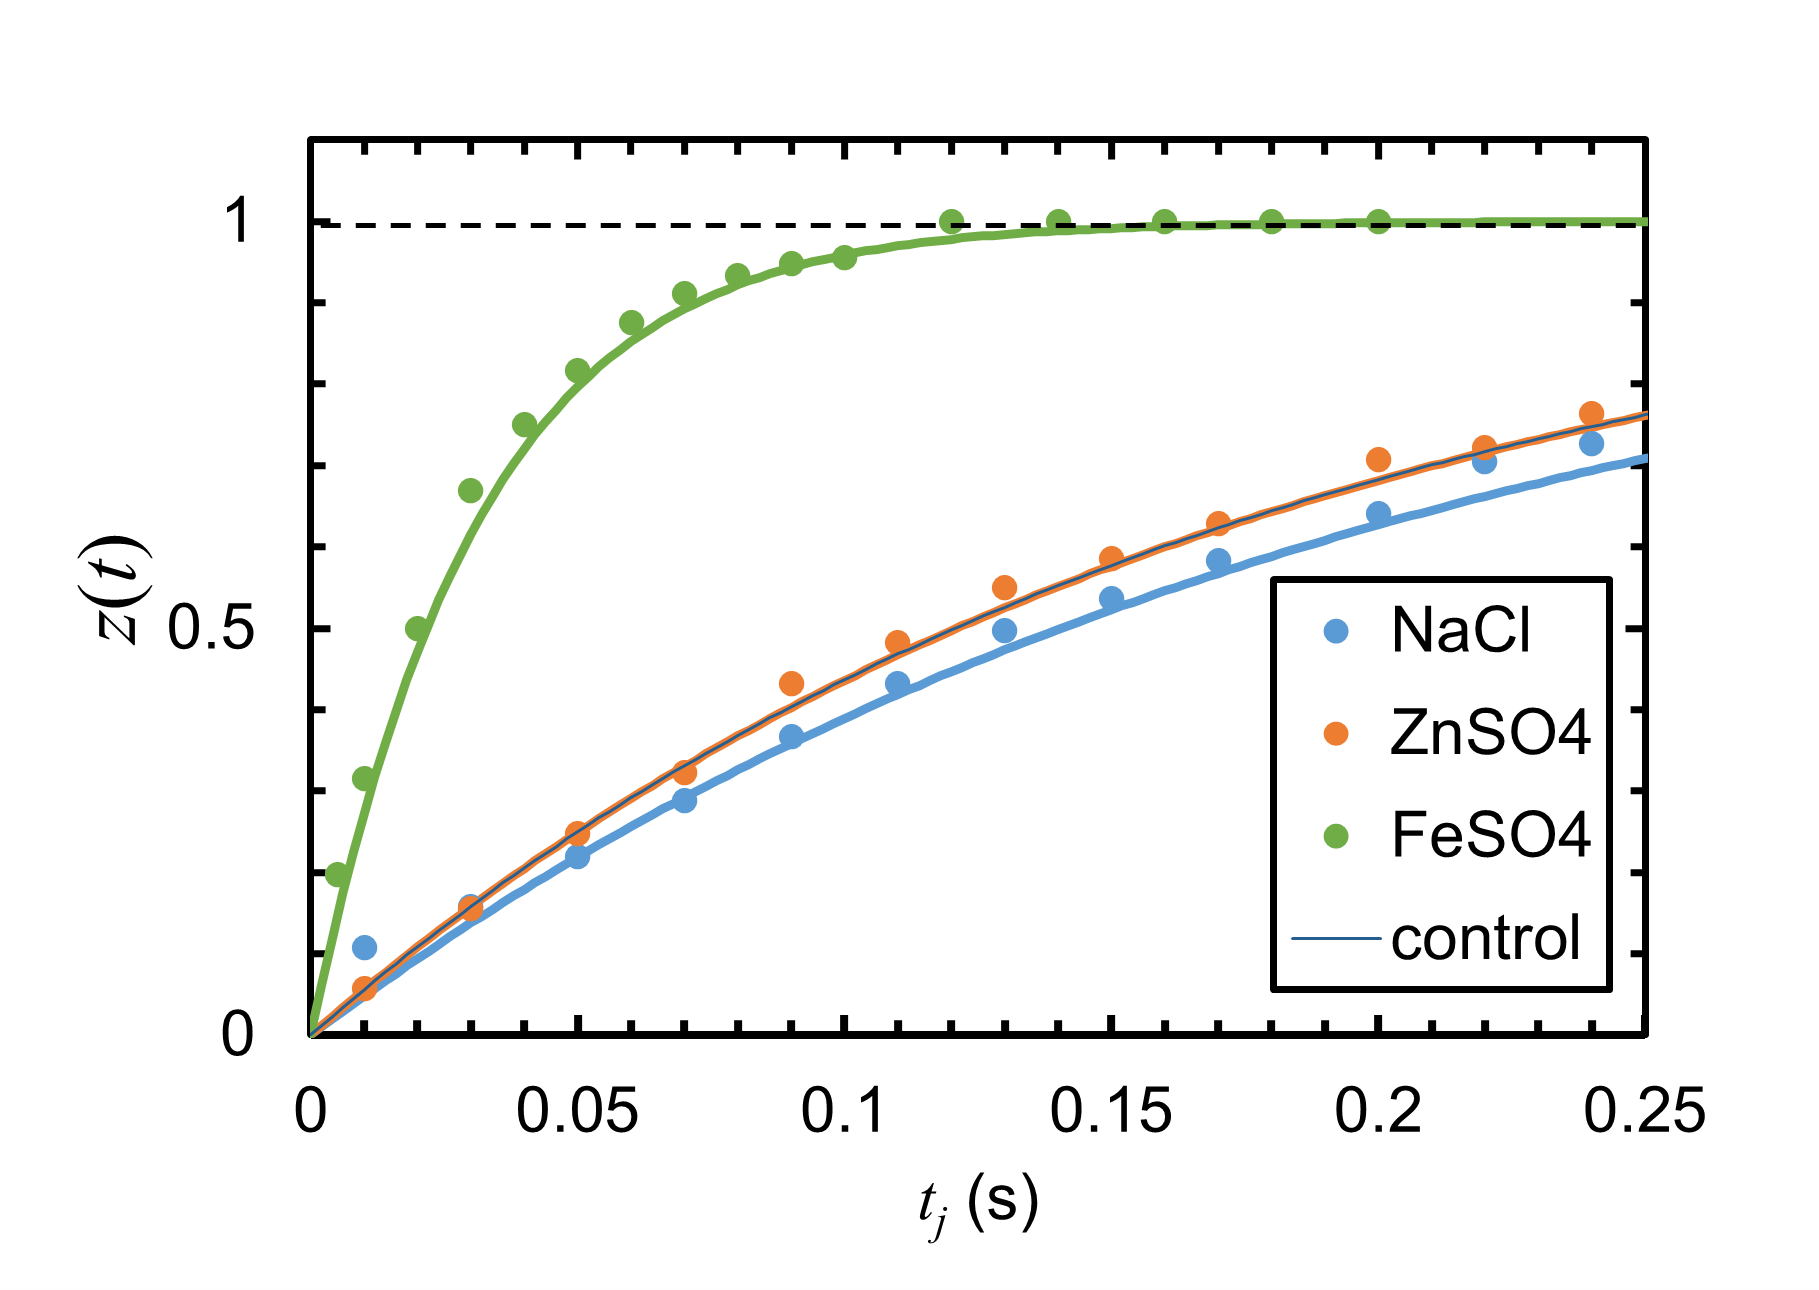
\includegraphics[width=\columnwidth]{graph/T1_var.png}
		\caption{\(5\times 10^{-3}\) mol/L \ce{CuSO4} 水溶液に各試料を入れたときの緩和の時間。
		control は何も入れていないときの緩和時間の変化を表していて、\ce{ZnSO4}のデータの重なっている。
		縦軸が状態\(\vb*{M}\)の\(z\)成分を表し、横軸が縦緩和の時間を表している。}
		\label{graph:T1_var}
	\end{minipage}
\end{figure}
\begin{figure}[h]
	\centering
	\begin{minipage}[t]{0.48\columnwidth}
		\centering
		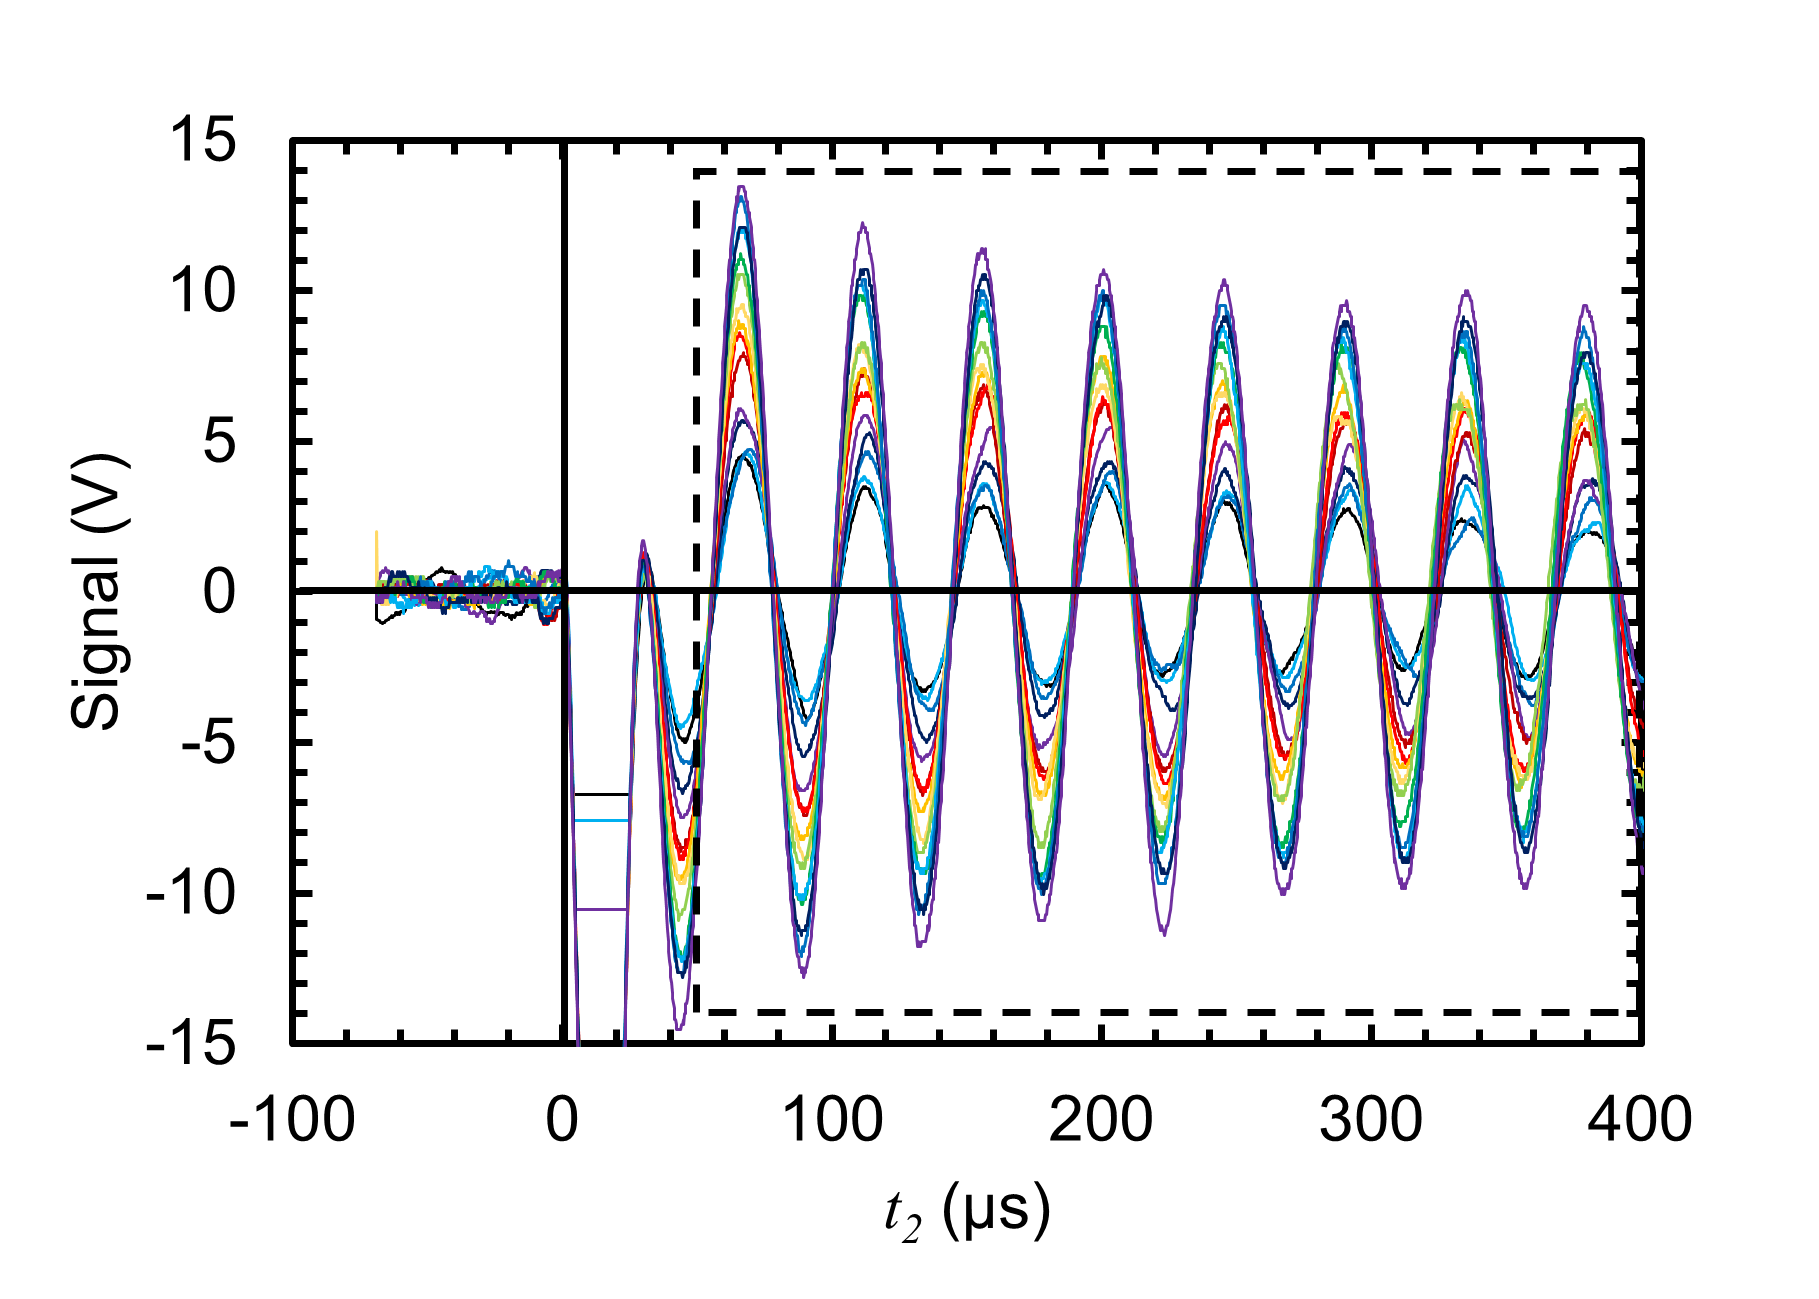
\includegraphics[width=\columnwidth]{graph/relaxation_water_ex.png}
		\subcaption{横緩和の測定結果}
		\label{graph:water_ex}
	\end{minipage}
	\hfill
	\begin{minipage}[t]{0.48\columnwidth}
		\centering
		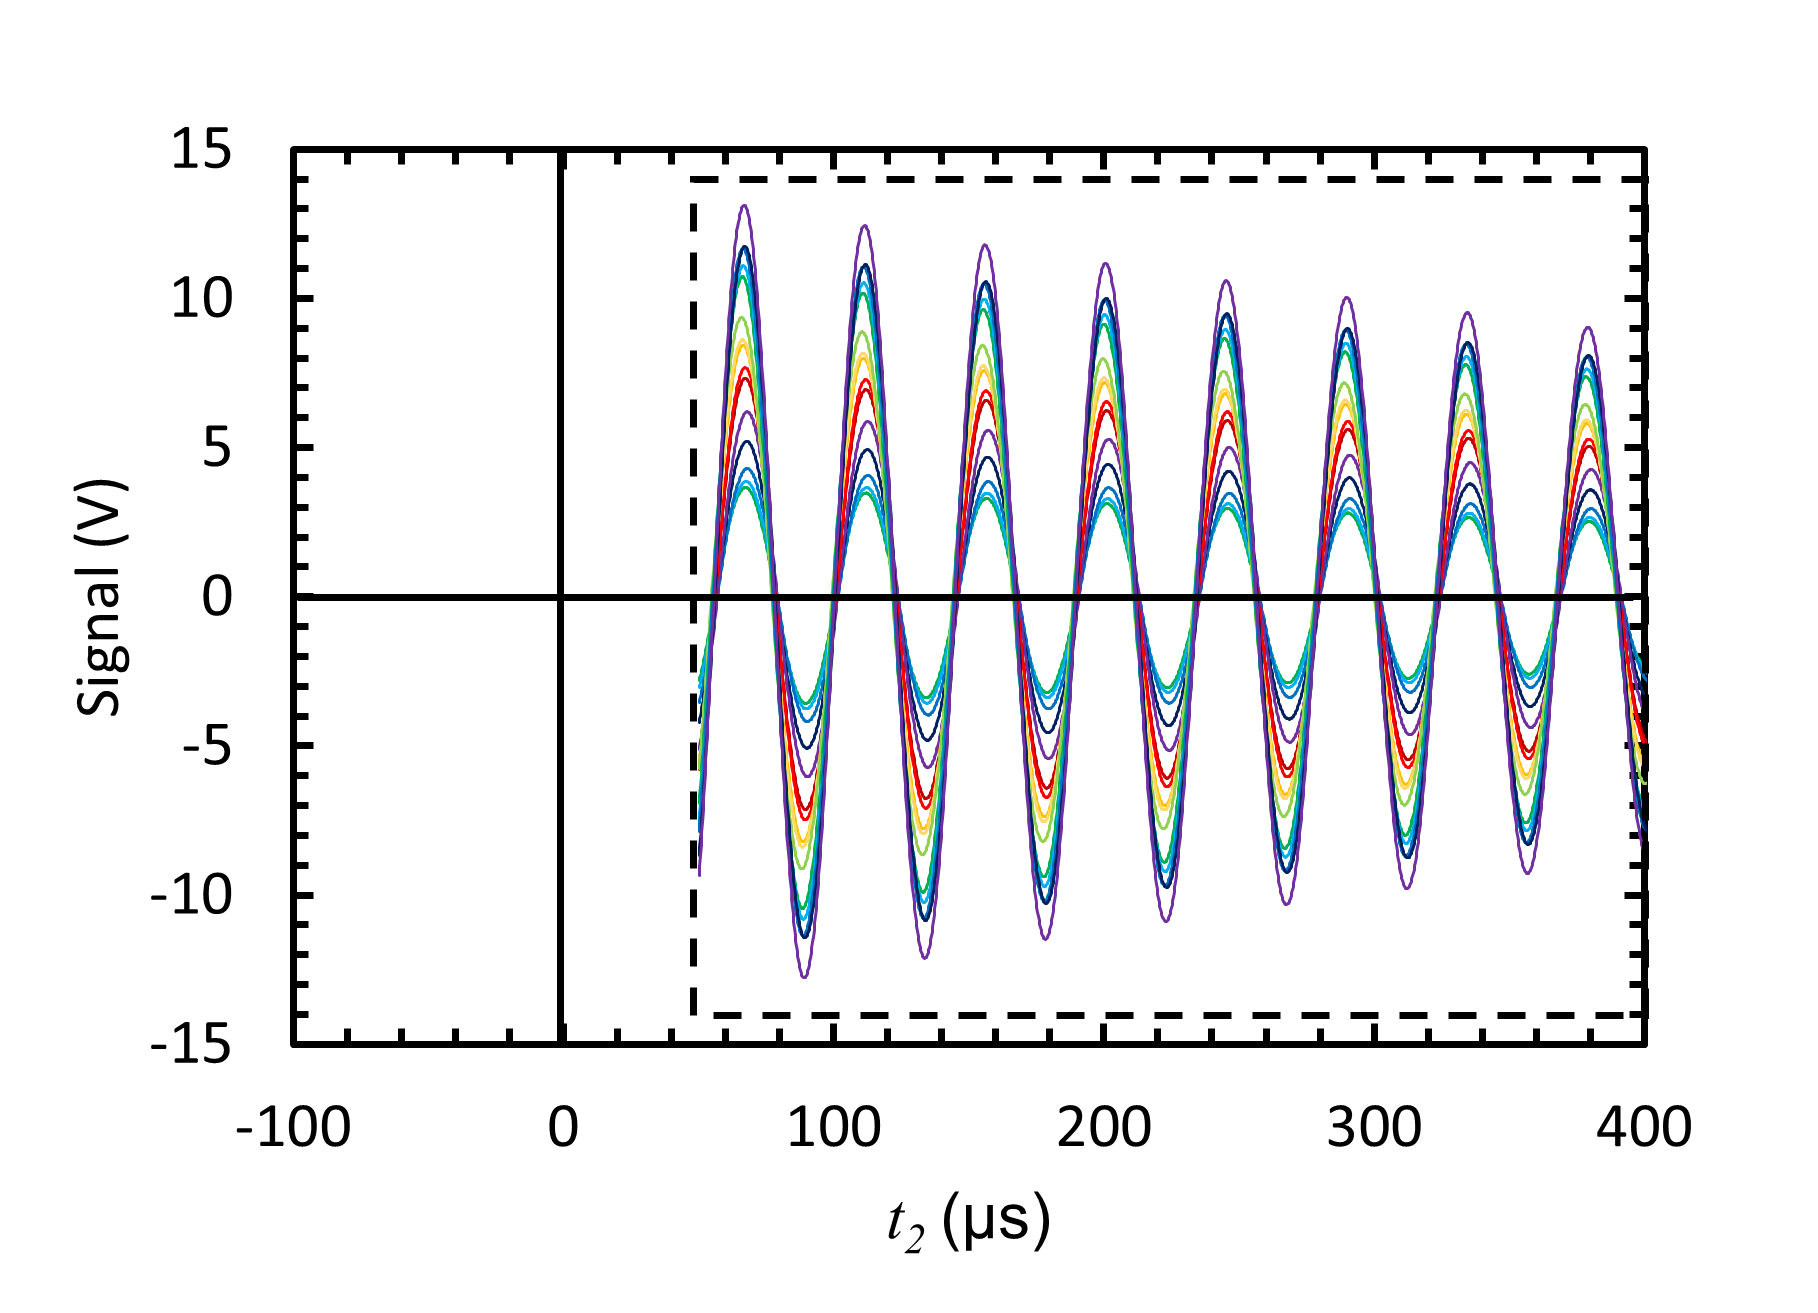
\includegraphics[width=\columnwidth]{graph/relaxation_water_fit.png}
		\subcaption{横緩和の測定をフィッティングしたもの}
		\label{graph:water_fit}
	\end{minipage}\\
	\begin{minipage}[t]{0.48\columnwidth}
		\centering
		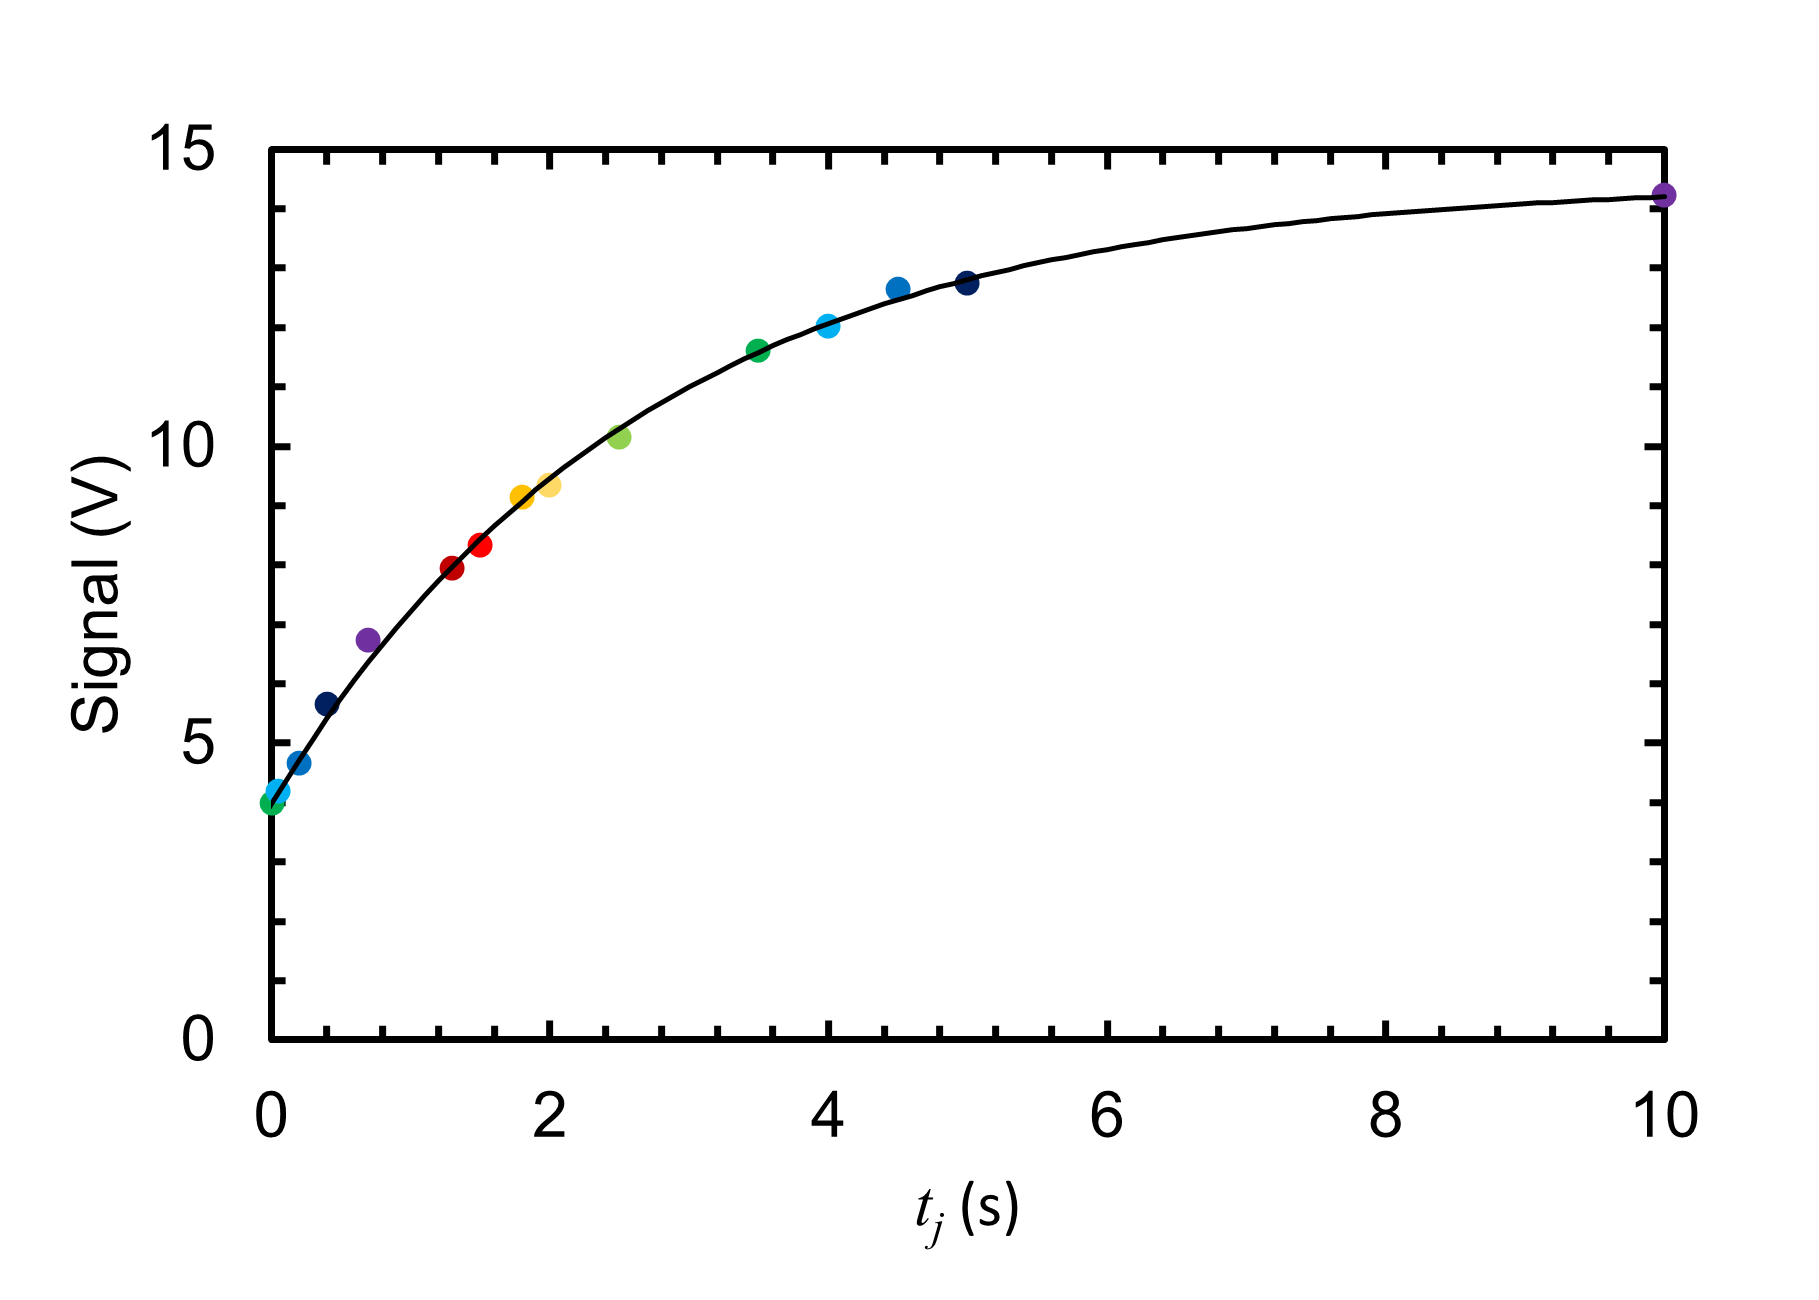
\includegraphics[width=\columnwidth]{graph/T1_water.png}
		\subcaption{横緩和の測定結果。縦緩和しきったか不明であるため、縦軸は装置の出力電圧にしてある。
		またフィッティング曲線は原点からの指数緩和ではなく、初期時刻からの指数緩和とした(考察)。}
		\label{graph:T1_water}
	\end{minipage}
	\caption{純水の緩和の様子。図\ref{graph:water_ex} は横緩和実験結果であり、
	二つの\(\pi/2\)パルスの間隔\(t_j\)を変えたときの出力波形をまとめてプロットしたものである。
	\(t_j\)が小さいときほど振幅(縦緩和の量)が小さいことがわかる。
	図\ref{graph:water_fit}は図\ref{graph:water_ex}のうち、
	点線で囲った領域を減衰振動としてフィッティングして得られた波形である。
	横緩和時間\(T_2\)や周期は同じものとして、
	\(T_2\), 周期、振幅、初期位相をフィッティングパラメータとした。
	そうして得られた振幅をプロットしたしたのが図\ref{graph:T1_water}である。}
	\label{graph:water}
\end{figure}
\begin{table}[h]
	\centering
	\caption{各試料中における水素原子核磁気共鳴の縦緩和\(T_1\)と横緩和時間\(T_2\).
	\ce{NaCl}, \ce{ZnSO4, \ce{FeSO4}} は \(5\times 10^{-3}\) mol/L \ce{CuSO4} 水溶液に入れたときのものである。
	- はデータがなく未測定。}
	\label{table:relax}
	\begin{tabular}{cccc}
		\hline\hline
		緩和時間 & \ce{CuSO4} (\(20\times 10^{-3}\) mol/L) & \ce{CuSO4} (\(10\times 10^{-3}\) mol/L) & \ce{CuSO4} (\(5\times 10^{-3}\) mol/L) \\
		\hline
		\(T_1\) (ms) & 49.4 & 87.5 &  174.2\\
		\(T_2\) (\si{\micro s})& - & - & -\\
		\hline \hline
		 & & & \\
		\hline \hline
		\ce{NaCl} & \ce{ZnSO4} & \ce{FeSO4} & 純水\\
		\hline
		202.8 & 174.7 & 31.4 & 2706.8\\
		- & - & - & 834.9\\
		\hline \hline
	\end{tabular}
\end{table}

% \newpage
\clearpage

\section{考察}
\subsection{純水の緩和}
\subsubsection*{2種類の縦緩和}
\subsubsection*{横緩和の原因}

\subsection{状態の緩和と情報}

量子情報の観点からスピンの状態の緩和を調べる。
始めは系全体のスピンの向きに関する情報を完全に持っている純粋状態であるため Bloch 球の球面に系の状態はあったが、
スピンがランダムな弾性散乱を受けるため、
系の持つ情報が失われていき、
状態が Bloch 球の球面にない混合状態へと向かっていくこととなる。
系が純粋状態であるか混合状態であるかの量は密度演算子\(\hat{\rho}\)の二乗のトレースをとるとわかる。
これを純度 (Purity) という。
 Purity \(\gamma_{\text{pure}}\)は二準位系においては\(1/2 \leq \gamma_{\text{pure}}\leq 1\)であり、
\(\gamma_{\text{pure}} = 1\)のときは純粋状態、そうでないときは混合状態である(証明略)。

この系における Purity の時間発展を求める。
Purity と Bloch ベクトルの成分の関係は
\begin{align}
	\gamma_{\text{pure}}(t) &= \tr[\hat{\rho}^2] \notag\\
	&=\frac{1}{4}\tr[
		\begin{pmatrix}
			1 + z(t) & \xi^*(t)\\
			\xi(t) & 1 - z(t)
		\end{pmatrix}^2]\notag\\
	&=\frac{1}{2}\qty(1+\xi^2(t)+z^2(t)) \notag\\
\end{align}
である。
これに緩和のある Bloch 方程式の解である(\ref{eq:relaxed_Bloch_sol})式を入れると、
\begin{equation}
	\gamma_{\text{pure}} = \frac{1}{2}\Bigl\{1+\xi_0^2e^{-2\gamma t}+\qty(z_0 e^{-\Gamma t} + z_{1}(1-e^{-\Gamma t}))^2\Bigr\}
\end{equation}
となる。
このパラメーターの振る舞いを見ると Purity の取るべき値の範囲より\(\Gamma < 2\gamma\)であることがわかる。
\footnote{\url{https://www.desmos.com/calculator/f53hirrjpr}で実際に Purity の振る舞いをパラメータを変化させながら見ることができる。}
これは緩和時間\(T_1 := 1/\Gamma,\,T_2 := 1/\gamma\)で表すと、
\begin{equation}
	T_2 \le 2T_1
\end{equation}
という関係が示せる。

\begin{figure}[htb]
	\centering
	\begin{minipage}[t]{0.48\columnwidth}
		\centering
		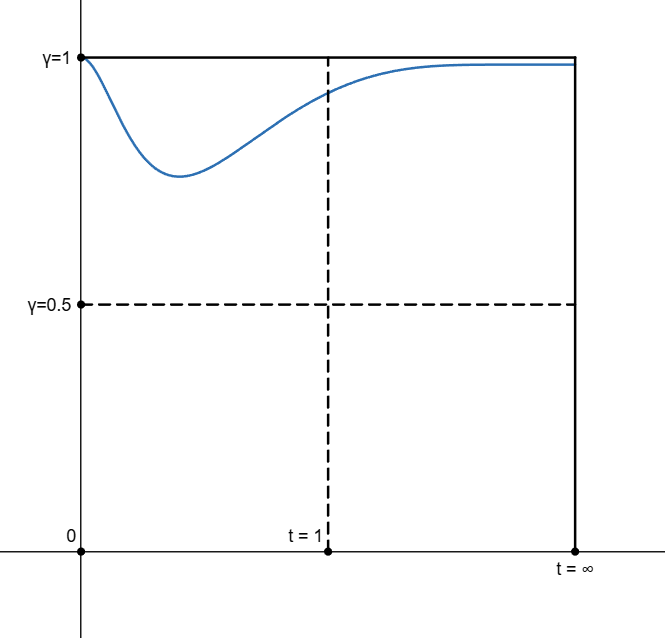
\includegraphics[width=\columnwidth]{/graph/purity_017.png}
		\subcaption{\(z_{1} \simeq 1\)の系が低温のとき}
	\end{minipage}
	\hfill
	\begin{minipage}[t]{0.48\columnwidth}
		\centering
		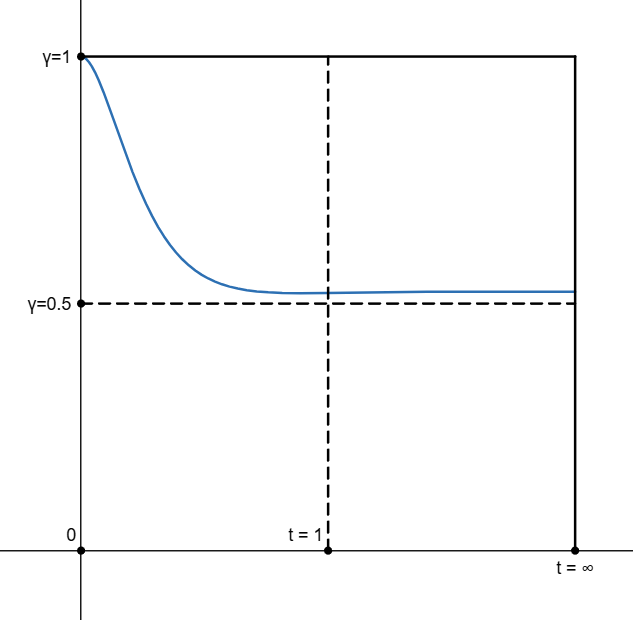
\includegraphics[width=\columnwidth]{/graph/purity_135.png}
		\subcaption{\(z_{1} \simeq 0 \)系がの高温のとき}
	\end{minipage}
	\caption{\(z_0 = 0,\, |\xi_0|=0,\,\Gamma=2.79,\,\gamma=2\)のときの
	 Purity \(\gamma_{\text{pure}}(t)\)のグラフ。
	 横軸は時間で無限遠での振る舞いを見れるように\(\tan t\)とした。
	 温度により変化する\(z_{1}\)により無限遠での Purity の値が変わり、
	 低温極限ではもともと外部にあった静磁場により情報が取り戻され、
	 高温極限では静磁場との相互作用がなくなるため情報が完全に失われることがわかる。}
	 \label{graph:purity}
\end{figure}

Purity の時間発展の様子と温度の関係を調べる。
初期状態\(\vb*{M}=(\xi_0,\,z_0)\)が純粋状態であるとする。
低温極限\(z_{1}=1\)では、
Purity は始めは 1 であったのが緩和により値が減少し、その後 1 に戻っていくのに対し、
高温極限\(z_{1}=0\)では最終的には 1/2 となる(図\ref{graph:purity})。
この振る舞いは次のように解釈される。

\(t=0\)では純粋状態であったが、
ここから横緩和\(\gamma\)によりこの状態は各々のスピンは\(z\)軸を回転軸としてランダムに回転し始め、
コヒーレンスを失っていくため\(\gamma_{\text{pure}}\)の値は小さくなっていく。
外部静磁場が温度による影響よりも強いような場合、
乱雑な向きになったスピンの向きは時間が経てば、
外部静磁場との相互作用によりスピンは\(z\)軸の方向へと揃っていきコヒーレンスが回復してくるため、
Purity は増加していく。
低温極限では温度ゆらぎがないため、
どのスピンも状態は\(\vb*{M}=(0,1)\)の上向きとなり、
系についての情報を完全に取り戻した純粋状態になる。
一方外部磁場が温度による影響よりも弱いときには、
磁場との相互作用によってスピンの向く方向を変えることができないため、
スピンの向く方向はそろうことなく Purity は下がっていく一方となる。
高温極限では外部磁場はないのと同じであるため、
スピンは完全に乱雑な方向を向き系についての情報を何も持たない\(\gamma_{\text{pure}}=1/2\)の完全混合状態となる。

\section{課題}
\subsection{水素原子核の磁気モーメントの大きさ}
\(I = 28.2\) A の電流を電磁石に流し \(0.298\) T の静磁場を
\(20\times 10^{-3}\) mol/L の硫酸銅(II)水溶液に加えた。
これによるエネルギー準位の Zeeman 分裂幅に対応する共鳴周波数は
\begin{equation}
	\omega_0 = 12.7  \text{Hz}
\end{equation}
であった。これにより陽子の磁気回転比\(\gamma_p\)は
\begin{equation}
	\gamma_p = 2.67 \times 10^8 \text{rad/T・s}
\end{equation}
とわかった。
これにより、陽子の磁気モーメントは
\begin{equation}
	\mu_p = 1.41 \times 10^{-26} \text{J/T}
\end{equation}
とわかった。
ボーア磁子は\(\mu_B = 9.27 \times 10^{-24} \text{J/T}\)であり、
で電子と陽子の質量比は 1840 程度であるため、陽子の\(g\)因子は
\begin{equation}
	g_p = \frac{m_p\mu_p}{m_e\mu_b}|g_e| =5.582
\end{equation}
と測定された。
CODATA の陽子の\(g\)因子の推奨値は
\begin{equation}
	g_p = 5.5856946893 \pm 0.0000000016
\end{equation}
である。
比較すると、今回の実験で得られた陽子の磁気モーメントの大きさはよいものだったとわかる。

\subsection{イオンの磁性}
イオンに磁性があるのは原子核の周りの電子に不対スピンがあるときである。
そうしたとき、スピンによる内部磁場により原子核の感じる磁場は強くなり、緩和時間は短くなる。
今回測定した試料中に含まれる原子の電子構造は表\ref{table:atom_structure}の通りである。
\begin{table}
	\centering
	\caption{測定した試料に含まれる原子とその電子構造。
	水素と酸素と硫黄は共有結合しているため不対電子がないとみなし省く。}
	\label{table:atom_structure}
	\begin{tabular}[t]{cl}
		\hline
		原子 & 電子構造 \\
		\hline \hline
		\ce{Na+} & \([1s^2][2s^2][2p^6]\)\\
		\ce{Cl-} & \([1s^2][2s^2][2p^6][3s^2][3p^6]\)\\
		\ce{Fe^2+} & \([1s^2][2s^2][2p^6][3s^2][3p^6][3d^6]\) \\
		\ce{Cu^2+} & \([1s^2][2s^2][2p^6][3s^2][3p^6][3d^6][3d^9]\) \\
		\ce{Zn^2+}& \([1s^2][2s^2][2p^6][3s^2][3p^6][3d^6][3d^9]\)\\
		\hline
	\end{tabular}
\end{table}

\subsection{硫酸銅(II)水溶液の濃度と緩和時間}

\subsection{純水の緩和}

\section{結論}


% J.J. Sakurai \cite{Sakurai_Napolitano_2020}
% Slichter \cite{Slichter_1990}

\bibliographystyle{junsrt}
\bibliography{reference}
\section*{付録}
% \section{摂動論}% もしかしたらまとめるかも

% \section{電子の \(g\) 因子の導出}

\section{量子光学}
この実験で扱った NMR の系は磁気双極子が外場である磁場の応答を見るという系になっている。
物質の光学応答を見る系は、電気双極子が外場である光電場に対する応答を見る系になっていて計算上の手続きはまったくと言っていいほど同じようにできる。
この節では松岡先生の書いた量子光学の教科書\cite{Matsuoka_2000}を参考にしながらまとめてみる。
\subsection{2準位系と密度演算子}
原子には電子の取ることができる準位が多数ある。
入射した光に共鳴するような状態を考えるときには、
入射した光の振動数に対応する2つの準位を取り上げれば十分である。
この2準位系にて電子がどう振る舞うかを考える。

まず基準となる2準位系を表すハミルトニアンを\(\hat{\mathcal{H}}_0\)とし、それらの固有状態と固有エネルギーを
\begin{equation}
	\hat{\mathcal{H}}_0 \ket{g} = E_g \ket{g}, \qquad \qquad \hat{\mathcal{H}}_0 \ket{e} = E_e \ket{e}
\end{equation}
のようにおく。
また行列表示の際には
\begin{equation}
	\ket{g} =
	\begin{pmatrix}
		0\\
		1
	\end{pmatrix}
	\qquad
	\ket{e} =
	\begin{pmatrix}
		1 \\
		0
	\end{pmatrix}
\end{equation}
として書く。
\footnote{\(g\)は ground state,\(e\)は excited state の頭文字である。}

この系に光電場\(\vb*{E}\)が入ってくるわけだがこの電場と系との相互作用は電気双極子によるものと考える。
このとき電気双極子モーメントは量子力学的に、光電場は古典的に扱う半古典論で考える。
電気双極子モーメント演算子を考える。
基底状態と励起状態では電子雲の描像で考えると原子は電荷の片寄りがない。
そのためその状態では原子は電気双極子モーメントを持たない。
一方状態が遷移しているときには電子雲は揺らいでいてこれにより電子双極子モーメントを持つと考える。
\(\hat{\vb*{r}}\)を電荷の位置とすると、
電気双極子モーメントの演算子は
\begin{equation}
	\hat{\vb*{\mu}} = q \hat{\vb*{r}}
\end{equation}
で表される。
これよりそこにできる双極子モーメントは
\begin{equation}
	\vb*{\mu}_{ge} = \bra{g}q\hat{\vb*{r}}\ket{e},\qquad \vb*{\mu}_{eg} = \vb*{\mu}_{ge}^{*}
\end{equation}
となる。
% \footnote{この演算子のによる電気双極子モーメントの描像は丁寧に記述された文献はあまりないように感じる。
% そのためあっているかは自信はあまりないものの、
% 自分の解釈では以上のような状態が量子力学的な電気双極子モーメントであると考えている。
% この描像は古典電磁気学的な電気双極子モーメントの描像と大分違うように感じる。}
これはお気持ち程度の解釈ではあるが、
厳密には多極子のパリティに関して Wigner-Eckart の定理というのがあり、
これにより\(\bra{g}\hat{\vb*{\mu}}\ket{g}\)といった対角成分は\(0\)になることがわかる。
摂動ハミルトニアン\(H_1\)は
古典電磁気学の双極子モーメントのポテンシャルエネルギー\(-\vb*{\mu}\cdot\vb*{E}\)を参考にして
\begin{equation}
	\hat{\mathcal{H}}_1 = - \hat{\vb*{\mu}}\cdot\vb*{E}
\end{equation}
となる。\footnote{光を量子化して電子と光子の相互作用の摂動を展開しても導出できる。
この展開により高次の多極子の相互作用についてかんがえることもできる。}
これによりハミルトニアンに非対角項が生じ、
基底状態から励起状態、励起状態から基底状態への遷移が起こるようになる。
以降摂動も含めた系のハミルトニアンを\(\hat{\mathcal{H}} := \hat{\mathcal{H}}_0 + \hat{\mathcal{H}}_1\)と書く。

この系を表す状態の時間発展を考える。
まず始めに状態ケット\(\ket{\psi}\)の表示から考える。
これらは摂動がないときの固有状態の線形結合としてかけ、
その線形結合の係数によって時間の様子を表すと考える。
よってこの系の状態ケットは
\begin{equation}
	\ket{\psi} = c_g (t) \ket{g} + c_e (t) \ket{e}
\end{equation}
と書ける。\(\rho_{gg}:=|c_g(t)|^2,\,\rho_{ee}:=|c_g(t)|^2\)という量はそれぞれの基底状態にある確率を表す。
また双極子モーメント演算子と合わせて使う際、状態の遷移を表すのに必要な量も導入する。
基底状態から励起状態への遷移は\(\rho_{ge} := c_g c_e^*\),
励起状態から基底状態への遷移は\(\rho_{eg} := c_e c_g^*\)
となる。
これらの量はまとめて行列として次のように表す。
\begin{equation}
	\hat{\rho} := c_g \ket{g}\bra{g} c_g^*
	+ c_g \ket{g}\bra{e} c_e^*
	+ c_e \ket{e}\bra{g} c_g^*
	+ c_e \ket{e}\bra{e} c_e^*
	=
	\begin{pmatrix}
		\rho_{ee} & \rho_{eg}\\
		\rho_{ge} & \rho_{gg}
	\end{pmatrix}
	=
	\begin{pmatrix}
		|c_g(t)|^2 & c_e c_g^*\\
		c_g c_e^* & |c_g(t)|^2
	\end{pmatrix}
\end{equation}
これを密度演算子(密度行列)と呼ぶ。
こういった系ではケットで状態を表すよりかは密度行列で表した方がよいので密度演算子で考える。
これの時間発展方程式を求めていく。

系の状態ケットをシュレディンガー方程式に入れると
\begin{equation}
	i\hbar\qty(\pdv{c_g}{t}\ket{g}+\pdv{c_e}{t}\ket{e}) = \hat{\mathcal{H}}\bigl(c_g (t) \ket{g} + c_e (t) \ket{e}\bigr)
\end{equation}
となる。この式の両辺に左から\(\bra{g},\,\bra{e}\)を掛けたものを行列を用いて表すと
\begin{equation}
	i\hbar\pdv{t}
	\begin{pmatrix}
		c_e\\
		c_g
	\end{pmatrix}
	=
	\begin{pmatrix}
		H_{ee} & H_{eg}\\
		H_{ge} & H_{gg}
	\end{pmatrix}
	\begin{pmatrix}
		c_e\\
		c_g
	\end{pmatrix}
\end{equation}
となる。
なので密度行列の成分\(\rho_{ij}\)の時間発展は
\begin{align}
	i\hbar\pdv{\rho_{ij}}{t} &= i\hbar\pdv{c_i}c_j^*+i\hbar c_i \pdv{c_j^*}{t}\\
	&= H_{ik} c_k c_j^* - c_i c_k^* H_{kj}\\
	&= (\hat{\mathcal{H}}\hat{\rho}-\hat{\rho}\hat{\mathcal{H}})_{ij}
\end{align}
よって密度行列の時間発展は
\begin{equation}
	i\hbar \pdv{t} \hat{\rho} = [\hat{\mathcal{H}},\,\hat{\rho}]
\end{equation}
と表わされる。(von Neumann 方程式)
また、導出は省くが密度演算子を使った物理量\(\hat{M}\)の期待値は
\begin{equation}
	\ev{\hat{M}} = \tr[\hat{\rho}\hat{M}]
\end{equation}
で表わされる。

\subsection{線形感受率}
外部電場に対する原子に束縛された電子ど原子核が作る分極の応答の関係を表す電気感受率を導出する。
2準位系の各準位のエネルギーを\(E_i = \hbar \omega_i\)のように書き、
共鳴する入射光の振動数を\(\omega := \omega_e -\omega_g\)とする。
また電気双極子モーメントは
\begin{equation}
	\vb*{\mu}_{ge}(t) = \bra{g}c_g^*(t)\,\hat{\vb*{\mu}}\,c_e(t)\ket{e}
	= \rho_{eg}\vb*{\mu}_{ge}
\end{equation}
である。この式を見ると密度行列の非対角成分の時間発展を追えばよいことがわかる。
この系のハミルトニアンは
\begin{equation}
	\hat{\mathcal{H}} =
	\begin{pmatrix}
		\hbar \omega_e  & -\vb*{\mu}_{eg}\cdot\vb*{E}\\
		-\vb*{\mu}_{ge}\cdot\vb*{E} & \hbar \omega_g
	\end{pmatrix}
\end{equation}
となる。これを von Neumann 方程式に入れて\(\rho_{eg}\)の時間発展を求めると
\begin{align}
	i\hbar \pdv{\rho_{eg}}{t} &= H_{ee}\rho_{eg} + H_{eg}\rho_{gg} - \rho_{ee} H_{eg} - \rho_{eg} H_{gg}\\
	\pdv{\rho_{eg}}{t} &= -i\omega_0\rho_{eg} -i\frac{\vb*{\mu}_{eg}\cdot \vb*{E}}{\hbar}(\rho_{ee}-\rho_{gg})
\end{align}
のようになる。
% 同様に\(\rho_{ge}\)についてもやると
% \begin{equation}
% 	\pdv{\rho_{ge}}{t} = i\omega_0\rho_{ge} +i\frac{\vb*{p}_{ge}\cdot \vb*{E}}{\hbar}(\rho_{ee}-\rho_{gg})
% \end{equation}
というのが得られる。
実際には\(\rho_{eg}\)は電気双極子モーメントに相当するため、これらの時間発展の式に緩和項を入れる。
すると
\begin{align}
	\pdv{\rho_{eg}}{t} &= -i\omega_0\rho_{eg} -\gamma\rho_{eg} -i\frac{\vb*{\mu}_{eg}\cdot \vb*{E}}{\hbar}(\rho_{ee}-\rho_{gg})\\
	\pdv{\rho_{ge}}{t} &=  i\omega_0\rho_{ge} -\gamma\rho_{ge} +i\frac{\vb*{\mu}_{ge}\cdot \vb*{E}}{\hbar}(\rho_{ee}-\rho_{gg})
\end{align}
となる。
ここから電気双極子と電場は z 成分だけを考え、電場は振幅と振動成分を分けて
\begin{equation}
	E(t) = E(\omega)e^{-i\omega t} + E(-\omega) e^{i\omega t} \label{eq:E_fourier}
\end{equation}
とする。\footnote{電場の位置依存性を調べたいときには\(e^{-i\omega t} \rightarrow e^{-i(\omega t +kz)}\)とする。}
また密度行列の非対角成分について、強制振動の系であることから
\begin{equation}
	\rho_{eg}(t) = \rho_{eg}^{(\omega)} e^{-i\omega t}
	, \qquad \rho_{ge}(t) = \rho_{ge}^{(-\omega)} e^{ i\omega t}  \label{eq:rho_fourier}
\end{equation}
というように置きなおすと便利になるであろう。これはちょうど振動数\(\omega\)で回転する系でこの現象を見るのと同じ変換になっている。
これはフーリエ変換した表示ではないので\(\rho_{eg}^{(\omega)}\)は時間に依存に注意することは必要である。
これらを時間発展の式に入れると
\begin{align}
	\pdv{\rho_{eg}^{(\omega)}}{t}
	  &= -i(\omega_0-\omega)\rho_{eg}^{( \omega)} -\gamma\rho_{eg}^{( \omega)} -i\frac{\mu_{eg}E( \omega)}{\hbar}(\rho_{ee}-\rho_{gg})-i\frac{\mu_{eg}E(-\omega)e^{ 2i\omega t}}{\hbar}(\rho_{ee}-\rho_{gg})\\
	\pdv{\rho_{ge}^{(-\omega)}}{t}
	  &=  i(\omega_0-\omega)\rho_{ge}^{(-\omega)} -\gamma\rho_{ge}^{(-\omega)} +i\frac{\mu_{ge}E(-\omega)}{\hbar}(\rho_{ee}-\rho_{gg})+i\frac{\mu_{ge}E(\omega)e^{-2i\omega t}}{\hbar}(\rho_{ee}-\rho_{gg})
\end{align}
\(e^{2i\omega t}, e^{-2i\omega t}\)の項は注目している振動数の第二高調波に相当するためこの項を無視する。
なので時間発展は
\begin{align}
	\pdv{\rho_{eg}^{(\omega)}}{t}
	  &= -i(\omega_0-\omega)\rho_{eg}^{( \omega)} -\gamma\rho_{eg}^{( \omega)} -i\frac{\mu_{eg}E( \omega)}{\hbar}(\rho_{ee}-\rho_{gg})\\
	\pdv{\rho_{ge}^{(-\omega)}}{t}
	  &=  i(\omega_0-\omega)\rho_{ge}^{(-\omega)} -\gamma\rho_{ge}^{(-\omega)} +i\frac{\mu_{ge}E(-\omega)}{\hbar}(\rho_{ee}-\rho_{gg})
\end{align}
と書ける。
このように回転する系の中で\(2\omega \)の項を無視する近似を回転波近似という。

誘電率を考えるときには定常状態とみなすため左辺の時間微分は 0 とみなす。
通常の光では励起状態に飽和するほどの光子は系に入らない。
2準位系のエネルギー差は eV オーダーなのに対し、熱ゆらぎは 10 meV のオーダーであるためであるため、
励起した電子はすぐさま基底状態に戻ると考えられる。
これより\(\rho_{gg} = 1,\,\rho_{ee} = 0\)とできる。
ここの値を適切に考えることでレーザー光のような強い光で飽和した状態を考えることもできる。

よって
\begin{align}
	\rho_{eg}^{(\omega)}
	&= \frac{\mu_{eg}}{\hbar}\frac{1}{\omega_0 - \omega - i\gamma} E( \omega)\\
	\rho_{ge}^{(-\omega)}
	&= \frac{\mu_{ge}}{\hbar}\frac{1}{\omega_0 - \omega + i\gamma} E(-\omega)\\
\end{align}
が得られる。
これより電気双極子モーメントの期待値は
\begin{align}
	\ev{\mu} &= \tr\qty[\hat{\vb*{\mu}}\hat{\rho}]\\
	&=\mu_{ge}\rho_{eg}+\cc\\
	&=\frac{\abs{\mu_{eg}}^2}{\hbar}\frac{e^{-i\omega t}}{\omega_0 - \omega - i\gamma} E( \omega)
	+ \cc\\
	&=\frac{\abs{\mu_{eg}}^2}{\hbar}\qty[
		 \frac{1}{\omega_0 - \omega - i\gamma}]
	E(\omega)e^{-i\omega t} + \cc
\end{align}
分極は\(P=N\ev{\mu}/V=\varepsilon_0\xi E\)より電気感受率は
\begin{equation}
	\xi(\omega) = \frac{\abs{\mu_{eg}}^2N}{\varepsilon_0\hbar V}\frac{1}{\omega_0-\omega -i\gamma}
\end{equation}
となる。

\subsection{光学的 Bloch 方程式の導出}
飽和状態のようなときには
密度行列の対角成分の時間発展を考える。
von Neumann 方程式を考える。
励起状態から基底状態に落ちる緩和を表す項として\(\Gamma\rho_{gg}\)を入れると
\begin{align}
	\pdv{\rho_{ee}}{t} &= -\Gamma\rho_{ee}+\frac{1}{i\hbar} \qty(H_{ee}\rho_{ee} + H_{eg}\rho_{ge}
	- \rho_{ee}H_{ee} - \rho_{eg}H_{ge})\\
	\pdv{\rho_{gg}}{t} &= \quad\Gamma\rho_{ee}+\frac{1}{i\hbar} \qty(H_{ge}\rho_{eg} + H_{gg}\rho_{gg}
	- \rho_{ge}H_{eg} - \rho_{gg}H_{gg})\\
\end{align}
となる。この右辺に(\ref{eq:E_fourier})式や(\ref{eq:rho_fourier})式等を入れて回転波近似を入れながら
整理していくと
\begin{align}
	\pdv{\rho_{ee}}{t} &= -\Gamma\rho_{ee} -\frac{i}{\hbar}
	\bigl\{-\mu_{eg}E(\omega)\rho_{ge}^{(-\omega)}
	+\mu_{ge}E(-\omega)\rho_{eg}^{(\omega)} \bigr\}\\
	\pdv{\rho_{gg}}{t} &= \quad\Gamma\rho_{ee} -\frac{i}{\hbar}
	\bigl\{-\mu_{ge}E(-\omega)\rho_{eg}^{(\omega)}
	+\mu_{eg}E(\omega)\rho_{ge}^{(-\omega)} \bigr\}
\end{align}
これら2式の差を取ると
\begin{equation}
	\pdv{t}(\rho_{ee}-\rho_{gg}) = - 2\Gamma\rho_{ee}
	- \frac{2i}{\hbar}\Bigl\{\mu_{ge}E(-\omega)\rho_{eg}^{(\omega)}
	-\mu_{eg}E(\omega)\rho_{ge}^{(-\omega)} \Bigr\}
\end{equation}
という時間発展の式が得られる。
% TODO 熱平衡状態についての記述

密度行列をSU(2)の直交基底
\((\hat{I},\,\hat{\sigma}_x.\,\hat{\sigma}_y,\,\hat{\sigma}_z)\)で展開することを考える。
密度行列の成分は回転座標系の下で
\begin{equation}
	\hat{\rho} =
	\begin{pmatrix}
		\rho_{ee} & \rho_{eg}^{(\omega)}\\
		\rho_{ge}^{(-\omega)} & \rho_{gg}
	\end{pmatrix}
\end{equation}
と書ける。Hilbert-Schmidt 内積をとると
\begin{align}
	w &= \tr [\hat{\rho}\hat{I}]
	= \qty(\rho_{ee}+\rho_{gg}) = 1\\
	x &= \tr [\hat{\rho}\hat{\sigma}_x]
	= \qty(\rho_{eg}^{(\omega)}+\rho_{ge}^{(-\omega)})\\
	y &= \tr [\hat{\rho}\hat{\sigma}_y]
	= i\qty(\rho_{eg}^{(\omega)}-\rho_{ge}^{(-\omega)})\\
	z &= \tr [\hat{\rho}\hat{\sigma}_z]
	= \qty(\rho_{ee}-\rho_{gg}).
\end{align}
これを用いると
\begin{equation}
	\hat{\rho} = \frac{1}{2}\qty(\hat{I}+x\hat{\sigma}+y\hat{\sigma}_y+z\hat{\sigma}_z)
\end{equation}
と書ける。この\(\vb*{R} := (x,\,y,\,z)\)というベクトルは大きさが 1 になっていて、
半径 1 の球面上の点を指す。このベクトルを Bloch ベクトル、その球を Bloch 球と呼ぶ。
% また、Bloch ベクトルの成分はスピン演算子の期待値になっているのがわかる。
% これはつまり磁気モーメントを古典的な矢印と見なしてもよいことがわかる。
実数となるように電場の位相をずらしてやると
\begin{equation}
	\mu E := \mu_{eg}E(\omega) = \mu_{ge}E(-\omega)
\end{equation}
というようにすることができる。
\(\vb*{R} = (x,\,y,\,z)\)の時間発展方程式は今までの結果を用いると
\begin{equation}
	\dv{t}
	\begin{pmatrix}
		x\\ y\\ z
	\end{pmatrix}
	=
	\begin{pmatrix}
		-\gamma & -(\omega-\omega_0) & 0\\
		\omega -\omega_0 & -\gamma & -2\mu E/\hbar\\
		0 & 2\mu E/\hbar & -\Gamma
	\end{pmatrix}
	\begin{pmatrix}
		x\\ y\\ z
	\end{pmatrix}
\end{equation}
と書ける。
これを緩和のある Bloch 方程式という。
\(\omega-\omega_0\)という成分は
回転する座標系における見かけの電場電場として取り込まれる。
その見かけの電場\({\vb*{\tilde{E}}}\)は
\begin{equation}
	\vb*{\tilde{E}} := \qty(2E,\,0,\,\frac{\hbar(\omega-\omega_0)}{\mu})
\end{equation}
となる。
緩和の項\(\Gamma,\,\gamma\)を 0 すると
BLoch 方程式は
\begin{equation}
	\dv{\vb*{R}}{t} = \frac{\mu}{\hbar}\vb*{\tilde{E}}\times\vb*{R}
\end{equation}
というように書ける。
これは NMR の系を古典電磁気学や半古典論に分析すると得られる式
\begin{equation}
	\dv{\vb*{M}}{t} = \gamma_g \vb*{\tilde{H}} \times \vb*{M}
\end{equation}
と同じものになっている。

% \subsection{Bloch ベクトルの古典電磁気学的な描像}

% \subsection{光の量子化}

% \subsection{Fermi の黄金律}

% \subsection{自然放出}

\end{document}